% AER-Article.tex for AEA last revised 22 June 2011
\documentclass[AER]{AEA}
\usepackage{bbm}
\usepackage{lscape}


% The mathtime package uses a Times font instead of Computer Modern.
% Uncomment the line below if you wish to use the mathtime package:
%\usepackage[cmbold]{mathtime}
% Note that miktex, by default, configures the mathtime package to use commercial fonts
% which you may not have. If you would like to use mathtime but you are seeing error
% messages about missing fonts (mtex.pfb, mtsy.pfb, or rmtmi.pfb) then please see
% the technical support document at http://www.aeaweb.org/templates/technical_support.pdf
% for instructions on fixing this problem.

% Note: you may use either harvard or natbib (but not both) to provide a wider
% variety of citation commands than latex supports natively. See below.

% Uncomment the next line to use the natbib package with bibtex 
%\usepackage{natbib}

% Uncomment the next line to use the harvard package with bibtex
%\usepackage[abbr]{harvard}

% This command determines the leading (vertical space between lines) in draft mode
% with 1.5 corresponding to "double" spacing.
\draftSpacing{1.5}

\begin{document}

\title{Aggregating Distributional Treatment Effects: A Bayesian Hierarchical Analysis of the Microcredit Literature}
\shortTitle{Bayesian Distributional Effects Aggregation}
\author{Rachael Meager\thanks{The London School of Economics and Political Science, Houghton St, London WC2A 2AE. r.meager@lse.ac.uk. Funding for this research was generously provided by the Berkeley Initiative for Transparency in the Social Sciences (BITSS), a program of the Center for Effective Global Action (CEGA), with support from the Laura and John Arnold Foundation. I am immensely grateful to Ted Miguel and the team at BITSS. I also thank Esther Duflo, Abhijit Banerjee, Anna Mikusheva, Rob Townsend, Victor Chernozhukov, Isaiah Andrews, Tamara Broderick, Ryan Giordano, Jonathan Huggins, Jim Savage, Andrew Gelman, Tetsuya Kaji, Michael Betancourt, Bob Carpenter, Ben Goodrich, Whitney Newey, Jerry Hausman, John Firth, Cory Smith, Arianna Ornaghi, Greg Howard, Nick Hagerty, Jack Liebersohn, Peter Hull, Ernest Liu, Donghee Jo, Matt Lowe, Yaroslav Mukhin, Ben Marx, Reshma Hussam, Yu Shi, Frank Schilbach, David Atkin, Gharad Bryan, Oriana Bandiera, Dean Karlan, Greg Fischer, and the audiences of many seminars for their feedback and advice. I thank the authors of the 7 microcredit studies, and the journals in which they published, for making their data and code public. All my code and data are accessible online at https://bitbucket.org/rmeager/aggregating-distributional-treatment-effects. The paper was pre-registered on the OSF at https://osf.io/tdvc8/ recognizing that pre-registration is different for a meta-analysis.}}
\date{\today}
\pubMonth{Month}
\pubYear{Year}
\pubVolume{Vol}
\pubIssue{Issue}
\JEL{}
\Keywords{}

\begin{abstract}
Expanding credit access in developing contexts could help some households while harming others. Microcredit studies show different effects at different quantiles of household profit, including some negative effects; yet these findings also differ across studies. I develop new Bayesian hierarchical models to aggregate the evidence on these distributional effects for mixture-type outcomes such as household profit. Applying them to microcredit, I find a precise zero effect from the 5th to 75th quantiles, and uncertain yet large effects on the upper tails, particularly for households with business experience. These quantile estimates are more reliable than averages because the data is fat-tailed.
\end{abstract}


\maketitle

Financial market expansions in the developing world have the potential to create winners and losers. Increasing access to credit in particular may have heterogeneous effects, both because borrowers differ in their investment opportunities and because of general equilibrium dynamics (Banerjee 2013, Kaboski and Townsend 2011). Proponents of financial interventions such as microcredit claim that the positive impact on high-productivity borrowers justifies continued market expansion; detractors claim that the resulting market "saturation" leads to exploitative lending practices which systematically harm the most vulnerable borrowers (Ahmad 2003, Roodman 2012). Although recent studies have estimated sets of quantile treatment effects to address this concern, existing meta-analyses of microcredit ignored these sets of quantile effects due to a lack of methodology to aggregate them (Meager 2019, Vivalt 2016, Banerjee et al 2015a). In this paper I develop new models to aggregate evidence on distributional treatment effects, and apply them to randomized trials of expanding access to microcredit.

% It really matters to figure out this question, because microcredit is big, but it is hard, because QTEs are hard.
%If increasing access to microcredit typically has heterogeneous effects within a community, and perhaps even negative effects for certain households, this has implications for policymakers.
Microcredit institutions reached 140 million low-income clients with a global loan portfolio worth 124 billion dollars in 2019, and the figure is growing yearly (Microfinance Barometer, 2020). At this scale, negative impacts for even a small subset of borrowers would be concerning, and several governments have curtailed microfinance operations ostensibly for this reason (Microfinance Focus 2011, Banerjee 2013, Breza and Kinnan 2018). Even if microcredit benefits all households, an unequal distribution of gains may affect social and political institutions (Acemoglu and Robinson 2008, Acemoglu et al 2015). Several randomized trials find evidence of negative effects at lower quantiles of household business profits, but others find zero or positive impact there and on higher quantiles of the distribution (Augsburg et al. 2015, Attanasio et al. 2015, Banerjee et al. 2015b, Crepon et al. 2015, Angelucci et al. 2015, Tarozzi et al. 2015, Karlan and Zinman 2011). Forming a broad consensus on the distributional impact of microcredit is difficult given the lack of power to estimate these effects (Leon and Heo 2009) and the possibility of substantial differences in effects across studies, often referred to as concerns about generalizability or "external validity". Yet despite these concerns, academics and policymakers need to understand the typical impact of microcredit, especially given this the potential for harm (Schicks 2013).


The main contribution of this paper is a method to aggregate the distributional impact of microcredit that addresses concerns about generalizability even in the presence of certain data features which -- though widespread in economics -- substantially complicate the use of existing econometric approaches. I work within the Bayesian hierarchical modelling framework because it specifies the potential for treatment effect heterogeneity as a parameter of interest in its own right, and uses that parameter to adjust the uncertainty about the typical impact across settings and likely impact in new settings (Rubin 1981, Gelman et al 2004, Gelman and Pardoe 2006). This approach is well-established in statistics and is increasingly used for evidence aggregation in economics (Chib and Greenberg 1995, Dehejia 2003, Hsiang, Burke and Miguel 2013, Vivalt 2016, Bandiera et al 2017, Meager 2019). Partial pooling models such as Empirical Bayes have also been used to borrow power across regions or sub-units when studying large geographic areas, or to combine multiple estimates within a study (Hull 2018, Chetty and Hendren 2018, Chetty, Friedman and Rockoff 2014). Yet within the hierarchical framework there are no established tools to aggregate distributional effects.\footnote{Even outside of the hierarchical framework, the economics literature on external validity and generalizability has focused on inference across different types of average effects, such as extrapolating the LATE to the ATE within similar settings, or adjustments based on correlations between observable and unobservable covariates (Heckman, Tobias, and Vytlacil 2001, Angrist 2004,  Angrist and Fernandez-Val 2010, Bertanha and Imbens 2014, Allcott 2015, Dehejia, Pop-Eleches and Samii 2015, Gechter 2015, Athey and Imbens 2016, Andrews and Oster 2018). }

% Why we have to do special mixture models 
In applying the Bayesian hierarchical framework to the distributional effects of microcredit, I confront several challenges that require a substantially new, tailored modelling approach. The first issue is that for the microcredit data, even the estimation of quantiles themselves is not straightforward because the business outcomes -- profit, revenues and expenditures -- have large spikes at zero which invalidate the quantile estimator's classical asymptotics (Mosteller, 1946). The sampling variance of the quantiles is no longer Gaussian, and more troublingly, is often estimated to be zero in the sample due to the large number of ties. Obtaining zero standard errors causes practical problems for evidence aggregation because the general treatment effect is typically estimated using a weighted average of the effects from each study, where the \emph{inverse} standard error enters the weight. Yet even if one does not face this problem, there is a second challenge: aggregating using potentially quite different weights at different quantiles can introduce quantile crossing -- the situation in which the point estimate of, say, the 50th quantile lies above the point estimate of the 60th quantile --  in the aggregate quantile effects. Thus, the inherent monotonicity constraint on the quantile function can be violated during the aggregation exercise even if it holds in the individual studies. 

My approach addresses both of these problems by directly modelling the distributions of household outcomes using a flexible set of parametric mixture models. I specify treatment effects on the parameters of the tailored density function and partially pool information on these effects across studies by placing a hierarchical structure on these treatment effects. Building these models relies on contextual economic knowledge of the variables at hand. For example, when we sample households in rural villages in India or Mexico and ask about their business profit, we ought to expect a spike at zero because not all households own businesses and nor do they necessarily operate their businesses in every period, often being engaged in seasonal agricultural labour for months at a time. In this context, household business variables are produced by an extensive-margin decision (to operate a business or not) followed by an intensive margin decision (how much to spend or invest once in operation) -- the spikes at zero are part of the data-generating process that can and should be modelled explicitly. 

To capture these data features, I develop a set of mixture probability density function (PDF) models, each of which has a point mass or "spike" of households at zero and a continuous tail distribution or "slab" on the rest of the real line.  I specify potential treatment effects on the probabilities that households find themselves in the tails versus the spike, and effects on features of the tails such as means and variances. Economic theory and prior data suggests that profits, expenditures, revenues and even consumer durables spending outcomes tend to have fatter tails than Normal distributions, so I consider models with either lognormal, Pareto, or a mixture of these two distributions for the continuous portions of these variables (Piketty 2015, Gabaix 2008, Roy 1950). I analytically compute and report the quantile treatment effects implied by the underlying parameters of the tailored PDFs by employing the method of Castellaci (2012); the posterior uncertainty on these transformed effects is automatically provided within the Bayesian framework. 

% FINDINGS 
Applying these models to seven randomized trials of expanding access to microcredit, I find a precise zero effect on household outcomes from the 5th to 75th percentiles. Above the 75th percentile, there is substantial probability of a large positive impact on most outcomes, but there is greater uncertainty around this effect due to heterogeneity within and across studies. There are no generalizable negative quantile treatment effects. These patterns hold regardless of whether one uses lognormal or Pareto tails, although the lognormal fits this data best. Moreover, my analysis shows that the tails of profit, revenues and business expenditures are so heavy that estimated average treatment effects and use of Gaussian asymptotics for averages are unreliable (Koenker and Basset 1978, Mosteller 1946). The majority of the right tail impact of microcredit and the heterogeneity across studies occurs within the group of households who had previous business experience.\footnote{In Appendix D I pursue a bounding exercise to show that the precise and generalizable impact at zero is unlikely to be due to low take-up of loans.} The resulting potential increase economic inequality even within the group of households who previously operated businesses implies that the social welfare effects of microcredit are likely to be complex.

% make a plug for general applicability of the methods here (echo the conclusion)
The models presented in this paper have broad applicability in economics beyond the microcredit literature. As a complement to the traditional approach in economics of writing review articles to summarize literatures, formal exercises to synthesize evidence improve power and prevent undue focus on the most extreme effects (Rubin 1981). Yet in economics, as in social science more broadly, contextual heterogeneity across study settings often makes it difficult to combine the evidence because the generalizability of the evidence is unknown (Allcott 2015, Bisbee et al 2016, Pritchett and Sandefur 2015). The hierarchical approach is broadly appropriate as it incorporates uncertainty about the heterogeneity in effects across studies, and provides some indication of the extent to which extrapolation across settings is appropriate. Moreover, there are many policy settings in which quantiles are implicated in policy directly, often because welfare or tax policies are explicitly concerned with distributional effects. My models are especially relevant when the data contains discrete point masses due to extensive margin decisions, and studies for which the outcome data is likely to be fat-tailed. 


% DATA AND CONTEXT
\section{Data and Context}
%What is the point of this section? It is so you can know: why I chose these studies. Why I chose these outcomes. Why I chose the ITT. Why I chose these covariates and this takeup analysis. and through all of that I need to share with you a basic view about microcredit in more detail than in the intro. Then you can trust me that I have narrowed this question down in an intelligent way such that you will care about the answers I can provide.


% I examine 7 RCTs of expanding access to microcredit and here's why I chose them this way.
To aggregate the evidence on the quantile treatment effects of microcredit, I use data from seven studies which meet the following inclusion criteria: the main intervention must be an expansion of access to microcredit either at the community or individual level, the assignment of access must be randomized, and the study must be published before February 2015 (the period of my literature search). The selected studies are: Angelucci et al. 2015, Attanasio et al. 2015, Augsburg et al. 2015, Banerjee et al. 2015b, Crepon et al. 2015, Karlan and Zinman 2011, and Tarozzi et al. 2015, six of which were published in a special issue of the \emph{American Economics Journal: Applied Economics}.\footnote{I focus on expanding access to microcredit because this is the intervention closest to the policy of subsidizing microfinance institutions (MFIs) or promoting interventions under the general umbrella of "microcredit". Other RCTs of microfinance tend to randomly vary certain characteristics of the loans themselves, which allows researchers to understand the impact of these features of the loans but complicates the inference on the general impact of the standard microcredit model (Field et al 2013). Karlan and Zinman 2009 expands access to consumer credit, but microcredit is often considered categorically different to consumer credit; see Banerjee 2013 for a deeper discussion of this.} I restrict the sample to randomized controlled trials (RCTs) because they typically have high internal validity for estimating causal effects, and they all consider a reasonably uniform and simple "expansion" treatment in this case.\footnote{While the set of studies here may not be a representative sample of all possible microcredit interventions, there is little reason to suspect publication bias in this literature. The papers here published a variety of results most of which were null. This leads to less risk of classical publication bias in which only "significant" results appear in the literature. However, it is still possible that these studies are not representative of the world. To address this issue requires substantially more structure and has thus far been ignored in the meta-analysis literature. This may be because such an exercise requires the development of aggregation techniques that can account for differential types of studies in a more complex way than a simple meta-regression, which fails to share information across the study types.}


% I examine both business and consumption variables because that can test the ways that microcredit was supposed to be a silver bullet
I analyse six outcomes linked to the claim that offering households more credit on more favourable terms should stimulate entrepreneurship (Morduch 1999, Yunus 2006, Roodman 2012). Because microfinance institutions (MFIs) offer lower interest rates relative to informal moneylenders, poor entrepreneurs may be able to start new businesses or grow their existing businesses, increasing their business expenditures, revenues and ultimately profits (Yunus 2006). Households could then increase their consumption in the medium and long run. Yet even households without business investment opportunities may use microloans to shift spending away from "temptation goods" (pleasurable yet harmful expenditures) and towards durable goods (Roodman 2012, Banerjee 2013). This could happen if microcredit increases a household's expectation of escaping poverty in the future, or solves a self-control problem (Banerjee and Mullainathan 2010, Banerjee 2013). In all cases I analyze the effect of expanding access itself, called the Intention to Treat Effect in the original studies (Banerjee et al 2015b). I do not pursue an instrumental variables strategy as network links and potential general equilibrium effects within villages means the Stable Unit Treatment Value Assumption (SUTVA) is likely to be violated at the household level (Banerjee 2013, Kinnan and Townsend 2012, Breza 2012).\footnote{To investigate the role of take-up in this context, I pursue a bounds analysis explained further in Appendix D.}

% Even within this selected sample there is much cross-study heterogeneity so that's why we need to use BHMs.
Despite the restrictive inclusion criteria, the selected studies still differ substantially in their implementations and local contexts. They cover seven different countries, they have different partner NGOs, offering similar but not identical loan contract structures with different interest rates and loan sizes, and they differ in terms of their randomization units - five randomized at the community level and two at the individual level - with various encouragement and sampling designs (see Appendix C for details). Given this heterogeneity across studies, heterogeneity in the resulting effects seems likely. However, the 95\% confidence intervals of the quantile effects do overlap across most of the studies, suggesting meaningful similarities across settings. In this context, where the generalizability of the evidence across settings is unclear ex-ante, the Bayesian hierarchical framework is an appropriately cautious way to proceed with evidence aggregation.

% Here's specifically how I constructed and standardized the variables

The open data policies of the \emph{American Economics Journal: Applied Economics} and \emph{Science} allow me access to the microdata from all of these experiments, such that I can standardize which quantiles I compute across studies and can construct each underlying variable in a uniform manner across studies. The variables were measured in different currencies, in different years, and over different time periods (this matters because these are all flow variables). I standardize all measurements to be USD PPP in 2009 dollars over a two-week period. Business variables require further standardization: to capture the potential for microcredit to allow individuals to open new businesses or to switch to operating any existing seasonal businesses throughout the year, households with no business or missing business data have profits imputed as zero. This was the decision made by the original authors of many of the seven studies, because the business creation channel is closely tied to the central claims of Yunus (2006), and dropping the missing values can lead to underestimating the business creation effects of microcredit if there are any. I employ this strategy throughout to business expenditures and revenues as well.\footnote{While it would be ideal to examine effects on other variables such as income and assets, the measurement and definition of those variables differed across the studies to such an extent that it is unclear how to aggregate them. This issue was noted in Meager (2019) and in my pre-registration: https://osf.io/tdvc8/} I also construct all profit variables in my analysis using reported revenues and expenditures data to minimize recall bias or rounding biases. Other than standardizing the construction of variables as much as possible, I have conformed to the decisions made by the original authors. \footnote{I have used the entire sample available in the online data sets except in Ethiopia: this study contained a cross-randomized family planning treatment. I use only the pure control and the pure microcredit samples, which is the conservative choice given that we do not know how microcredit interacts with family planning (the study estimates a very imprecise interaction).}\footnote{I do not winsorize any of the variables because most of the original studies did not winsorize themselves. However Augsburg et al (2015) found that winsorizing outliers sometimes made results statistically significant when they were not significant in the full sample. If the extreme values do not change the point estimate but increase the uncertainty, winsorising them may underestimate the true uncertainty.}


% Here's why I deicded to do what I did on covariates and ITT. We have limited covariates available to us in this literature but I do what I can.
Household and study-level covariates may play some role in determining heterogeneity in the quantile treatment effects, but there are limitations to pursuing a covariates analysis in this literature. Only three of the microcredit RCTs collected comprehensive individual-level baseline surveys. One pre-treatment variable was recorded at endline in all studies due to its theoretical importance: a binary indicator that a household had previous experience operating a business (Banerjee et al 2015b). Although covariates at the study level may also predict variation in effects across context, there at least seven such covariates and only seven studies, so conventional regression analysis will be overfitted and misleading. It is still useful to aggregate the evidence without conditioning on covariates, as this permits an understanding how much unconditional heterogeneity there is; if there is little or no variation across settings, further analysis is a less pressing concern for future work.

% what is the heterogeneity kenneth? The Bayesian framework... what KIND of heterogeneity?
The main analysis that follows is therefore accounting for all sources of heterogeneity including differences in MFI policies, study design, measurement protocols, and contextual factors in the local economies. I do not attempt to separate out these different kinds of heterogeneity both because it is substantially challenging with 7 data points and because it is unclear if they can or should be separated. MFI policies, study design and even measurement protocols may all be endogenously determined by the MFI and researchers in response to the different contextual factors. Indeed, a team of researchers and a single MFI applying the exact same decision rules in which they optimally determine say interest rates or measurement protocols conditional on contextual factors would generically make different decisions in different contexts. Adjusting for the "measurement protocol" before applying the Bayesian model could therefore create differences across settings where none exist in the raw data. I therefore refrain from adjusting for any sources of heterogeneity a priori in the analysis that follows.

\section{Methodology}\label{methodology}

\subsection{Bayesian Hierarchical Models}

\subsubsection{Hierarchical Models}

%  this section defines a general methodological framework, generalized from the BHMs in Rubin, Gelman, Meager
Consider a body of evidence consisting of $K$ studies indexed by $k$, each of which provides some $k$-specific data $\mathcal{Y}_k$ about a given policy intervention. The $K$ data sets taken together form one large data set, denoted $\mathcal{Y} = \{    \mathcal{Y}_k \}_{k=1}^K$. Each study setting has a site-specific parameter of interest $\theta_k \in \Theta_k$, which could be univariate (e.g. the average treatment effect), or multivariate (e.g. the entire set of quantile treatment effects). The full data in each site $k$ consists of $N_k$ households, summing to $N$ households in the total combined sample of all settings.

Suppose that the analyst wishes to learn about the expected value of these  $\{\theta_k\}^K_{k=1}$ parameters across different settings, and to learn about the uncertainty she should have due to unobserved differences across settings. This implies a need for inference on the average value of these parameters, sometimes called the "hypermean" and denoted $\theta = E[\theta_k]$ with the expectation taken across the study settings. Accounting for uncertainty across settings permits inference not just to unobserved households in the existing sites but to unobserved study sites themselves, and thus, such a procedure could generate inference applicable beyond the current set of studies to future policy settings if such extrapolation is warranted.  

 One can learn about $\theta$ using the evidence on $ \{ \theta_k \}_{k=1}^K$, but the optimal learning procedure depends on the heterogeneity or dispersion of $ \{ \theta_k \}_{k=1}^K$ around $\theta$, denoted $\Sigma_{\theta}$ (Rubin 1981, Gelman et al. 2004). This $\Sigma_{\theta}$ describes the strength or weakness of the relationship between any $\theta_k$ and the general parameter $\theta$: if the dispersion $\Sigma_{\theta}$  is small, then $\theta_k$ is close to $\theta$ and provides a strong signal of the value of $\theta$. By the same logic, when $\Sigma_{\theta}$ is small then $\theta$ is a strong predictor of $\theta_{K+1}$ for some future setting.\footnote{Technically the sites must be "exchangeable", this condition is discussed in the final paragraph of this section.} Here $\Sigma_{\theta}$ parameterizes a notion of generalizability of the evidence contained in $\mathcal{Y}$ to external settings, which captures the definition of external validity in Allcott (2015) and Dehejia, Pop-Eleches and Samii (2015). If $\Sigma_{\theta} = 0$, then $\theta$ is a perfect predictor of $\theta_{K+1}$; if not, there will be some extrapolation error which grows large as the parameter $\Sigma_{\theta}$ grows large.

%  hierarchical models are good
Joint estimation of $\theta$ and $\Sigma_{\theta}$ is the core challenge of aggregation across studies. Hierarchical models approach this problem by defining a set of parameters at the site level, $\{ \theta_k\}_{k=1}^K$, a set of parameters at the population level, $\theta$, and a relationship between them (Efron and Morris 1975, Rubin 1981, Gelman et al. 2004). The "lower level" of the model describes the dependence between the data and local parameters in site $k$:
\begin{equation}
\begin{aligned}
\mathcal{Y}_k \sim f(\cdot | \theta_k) \; \forall \; k.
\end{aligned}
\label{lower level likelihood}
\end{equation}
The "upper level" of the model describes the potential for statistical dependence between local parameters and general parameters (also called "hyperparameters") via some likelihood function $\psi(\cdot)$, which contains the hypervariance $\Sigma_{\theta}$ either implicitly or explicitly depending on the specific model. While $\psi(\cdot | \theta, \Sigma_{\theta})$, this second argument is often implicit and thus notationally suppressed. This upper level "general" or "parent" distribution is then denoted:
\begin{equation}
\begin{aligned}
\theta_k \sim \psi(\cdot | \theta) \; \forall \; k.
\end{aligned}
\label{upper level likelihood}
\end{equation}
A hierarchical likelihood contains both levels: \begin{equation}
\begin{aligned}
\mathcal{L}(\mathcal{Y} | \theta) = \prod_{k=1}^K f(\mathcal{Y}_k | \theta_k)\psi(\theta_k | \theta).
\end{aligned}
\label{hierarchical likelihood}
\end{equation}

This likelihood structure nests both the "no pooling" case in which no information is shared across settings, and the "full pooling" aggregation case in which all information is shared fully across settings as if they are indistinguishable. This nesting is possible because the hyperparameters that govern the $\psi(\cdot)$ function, including $\Sigma_{\theta}$, are estimated rather than imposed. For example, the model may estimate that $\theta_k \approx \theta_{k'} \; \forall \; k, k'$, and hence that $\Sigma_{\theta}= 0$, if that is supported by the data. This result would recover the full-pooling model's solution, up to a degrees of freedom correction.\footnote{This discussion is in reference to models for estimating the average effects across the different settings, with uncertainty intervals referring to extrapolation to an unobserved setting. The full pooling model has another function: it can serve to estimate the average effect across all the individuals in the existing settings, with uncertainty intervals referring to an extrapolation to an unobserved individual within these given settings. This distinction is discussed further in the results section.} Of course, the model could detect large dispersion in $  \{\theta_k\}_{k=1}^K$; in that case it recovers the no-pooling model's solution. In fact, this model can recover a solution anywhere on the spectrum between these two extremes if that intermediate or "partial pooling" solution is most supported by the data. Inference on $  \{\theta_k\}_{k=1}^K$, $\theta$ and $\Sigma_\theta$ is influenced by the extent of this partial pooling, which is also called "shrinkage" because the $  \{\theta_k\}_{k=1}^K$ estimates are somewhat "shrunk" together when information is shared across settings.

% 1 PARGARAPH TO DISCUSS EXCHANGEABILITY HERE (do i want to have this fight here??????? can i have this fight later?)
Hierarchical models require that $\{{\theta}_k\}_{k=1}^K $   be ``exchangeable'', such that their joint distribution is invariant to permutation of the indices (Diaconis, 1977). This means the analyst must be ignorant of any definite ordering, dependence or sub-clustering of the parameters \emph{a priori}; this is the case for the microcredit effects as in most applications to social science. Knowledge of contextual differences typically does not inform us \emph{ex ante} of how $\theta_k$ parameters differ (Rubin 1981).\footnote{If an established and verified economic theory dictates that a particular covariate can only be correlated in a certain way with the treatment effects, that can be translated into $conditional$ exchangeability by introducing this covariate into the model. It is also possible to build a more complex structure that allows "partial exchangeability" if this is desired; see Albert and Chib (1997) for a discussion of this approach.}  The extensive theoretical literature on microcredit markets does not dictate a specific ordering of effects in this case, which makes exchangeability a reasonable structure (Gelman et al. 2004). Any future site for which $\theta_{K+1}$ is used to predict the effect must be exchangeable with the sites in the sample; this is a general requirement for any out-of-sample prediction (see for example Allcott 2015).

% DISCUSS THE ESTIMANDS FULL VS PARTIAL POOLING HERE , link back to it in the results discussion as bring DIFFERENT ESTIMANDS 


\subsubsection{Bayesian Implementation}

% priors are good for you like vegetables
Bayesian inference offers several advantages for the analysis of hierarchical models, particularly when aggregating across a relatively small number of studies, as is typically the case in economics. With seven microcredit studies, estimation of the variation in effects across settings is performed off only seven contexts. Given this low-data environment, incorporating informative Bayesian priors can substantially improve the performance of the hierarchical model by "regularizing" the likelihood problem in the classical sense: introducing new information that constrains the fit of the model, typically trading off bias for variance to reduce overall mean squared error and out-of-sample prediction (Hastie, Tibshirani and Friedman 2009, section 10.2; Chung et al. 2013, 2015). 

The inference proceeds by specifying a prior on the unknowns at the highest level, $\mathcal{P}(\theta)$, and combining it with the likelihood via Bayes' rule to generate the joint posterior distribution $f(\theta | \mathcal{Y}) $. The specification of a proper prior distribution ensures that $f(\theta | \mathcal{Y}) $ is a proper probability distribution with desirable decision-theoretic properties such as consistency and admissibility (Berger 2013, Van der Vaart 1998, Efron 1982). 

% posterior predictive distribution!!!! for theta_K+1} this really belongs here because WHO ELSE Can integrate over these parameter distributions? MOBODY
The Bayesian approach also automatically delivers the correct marginal distribution of the treatment effect in a hypothetical future site $\theta_{K+1}$. This is often the object of most interest for policymakers, but the distribution of this object must account for the full joint posterior uncertainty on the hyperparameters rather than conditioning on a particular point estimate.\footnote{The full joint posterior uncertainty accounts perfectly for the uncertainty about how well the new location matches the old location, if the new site is exchangeable with the old sites, and the model structures are correct. If these conditions do not hold, we have modeling uncertainty, which is not accounted for in any meta-analytic methods at present (nor in any of the popular analytic methods used in empirical economics).}The Bayesian approach delivers the correct uncertainty interval conditional on the model in the form of posterior predictive inference (Gelman et al. 2004), which averages over the posterior uncertainty on the unknowns $(\theta, \Sigma_{\theta})$. Formally, the posterior predictive distribution is:
\begin{equation}
\begin{aligned}
f(\theta_{K+1} | \mathcal{Y}) = \int \psi(\theta_{K+1} | \theta)f(\theta | \mathcal{Y})\text{d} \theta
\end{aligned}
\label{posterior predictive}
\end{equation}

% introduce and define a general bayesian structure (plus brief plug/explain why good)
The characterization of the full joint posterior distribution on all parameters is not without costs: it can exacerbate the already-formidable tractability issues inherent in hierarchical models. The relationships between $\theta$, $\Sigma_{\theta}$ and $\{\theta_k \}_{k=1}^K$ are highly nonlinear, leading to challenges optimizing and even characterizing the shape of the likelihood function. Common maximum likelihood approaches estimate the upper level first and then condition on the point estimates using the "empirical Bayesian" approach from Efron and Morris (1975). This ignores the uncertainty about the upper level parameters, $\theta$ and $\Sigma_{\theta}$, when computing uncertainty intervals on the lower level parameters, and thereby systematically underestimates uncertainty (Rubin 1981).\footnote{While MLE methods that do not condition on point estimates of unknowns are theoretically available, they seem to be largely unused in practice.} To surmount these tractability issues in the Bayesian setting I turn to Markov-Chain Monte Carlo methods; in particular, I use Hamiltonian Monte Carlo (HMC) methods which are well-suited to the peculiar geometry introduced by hierarchical structure (Betancourt and Girolami, 2013).\footnote{HMC uses discretized Hamiltonian dynamics to sample from the posterior, which can be combined with the No-U-Turn sampling method (NUTS) to auto-tune the step sizes in the chain (Hoffman and Gelman, 2014). This algorithm is automated in the software package Stan, a free statistical library which calls C++ to fit Bayesian models from R or Python (Stan Development Team, 2017).}

\subsection{Tailored Mixture PDF Models for Distributional Effects}

\subsubsection{Challenges of Distributional Effect Aggregation}
Applying the Bayesian hierarchical framework to distributional effects aggregation poses additional challenges which demand new modelling approaches. If one were interested in only a single quantile treatment effect, such as the median, one could directly apply a Rubin-style model to the quantile as long as the data meets the condition for the Mosteller (1946) theorem providing consistency and asymptotic Normality of the sample quantile estimate. However, for the microcredit data, even the estimation of quantiles themselves is not straightforward because many households outcomes are not continuously distributed (as required by the theorem), but instead have point masses of households at zero. The sampling variance of the quantiles is no longer Gaussian, and may even be estimated as zero in the finite sample (as in Angelucci et al 2015). Even if researchers are willing to accept zero estimated sampling error, this causes difficulties for a Rubin-style approach, which constructs weighted averages of estimated effects in which the \emph{inverse} standard error enters the weight.\footnote{It might be possible to overcome this problem by investigating CDF effects rather than quantiles, but applied researchers are directly interested in quantiles, and the transformation between CDFs and quantiles is not straightforward in the partially discrete data case.}

Moreover, aggregating sets of quantiles requires facing the constraint that the true quantiles must be monotonically increasing, because CDFs are monotonically increasing by definition. Violating this constraint leads to the "quantile crossing" problem, which can arise even in simple analyses (see for example Chernozhukov, Fernandez-Val and Galichon 2010). Aggregation exacerbates this problem because most methods both estimate the aggregate effect and revise the site-specific effect estimates by incorporating information on the local variation or sampling uncertainty, and this can be different at different quantiles across the different sites.  But differentially-weighted averages of monotonic functions need not themselves be monotonic, so the aggregation procedure could introduce quantile crossing where none was present in the original studies.\footnote{While it is possible to derive an aggregation model for sets of quantiles based on the Mosteller approximation that respects the logical properties of the estimands via variable transformation (see Appendix A), even this model would only be applicable to data for which the asymptotic theorem applies. In some cases of discrete data, such as with count data, it is possible to "dither" or "jitter" the discrete data to produce a new, continuous distribution for which the quantiles have a one-to-one relationship with the discrete distribution (Machado and Santos Silva, 2005). This does not work in the case of a partially discrete "spike and slab" distribution because the dithered data points from the spike generally leapfrog some of the data in the slab, destroying the one-to-one relationship between the quantiles.}

% my approach is THIS in a nutshell
\subsubsection{Tailored Mixture PDF Approach}
I address both of these problems by directly modelling the distributions of these outcome variables using a flexible set of mixture probability density functions (PDFs). These models specify treatment effects on the parameters of the tailored density function and partially pool information on these effects across studies by placing a hierarchical structure on these treatment effects. The conceptual approach is here is quite general, and even the specific models below are likely to apply beyond the microcredit application. In every case, however, building these parametric models relies on contextual economic knowledge of the variables at hand, and researchers must understand the data generating process well enough to know when it ought to exhibit, say, discreteness, skewness or kurtosis. The incorporation of this specific contextual knowledge is critical to the modelling process, as follows. 

Consider the household business variables in the microcredit data, generated by surveying a random sample of households. In most contexts, not all households will choose to own businesses, nor will they necessarily operate businesses they do have at all times, as they often do seasonal agricultural or manual labour for part of the year (Macours and Vakis 2010, Gibson and McKenzie 2014, Fink, Jack and Masiye, 2014). So measured business variables should be mixture of a discrete mass at zero and continuous tails, because these variables are the output of a partially discrete decision process. First, a household has an extensive margin decision to make about whether to start a business, and then they face a secondary extensive margin decision about whether to operate that business in a given season. Only those households who decide to open and operate their businesses go on to make an intensive margin decision, the result of which manifests some continuous expenditures, revenues and profit. In fact, this pattern also arises in consumer durables spending and temptation goods spending, to a lesser extent.  

I therefore use a set of mixture models to model this partially-discrete data, each of which has a point mass or "spike" of households at zero and a continuous distribution or "slab" on the rest of the real line. Economic theory and prior research further suggest that the continuous portions of business variables such as revenues and profit will tend to follow power laws or other fat-tailed laws (Roy 1950, Stiglitz 1969, Gabaix 2008, Allen 2014, Piketty 2015, Bazzi 2016). Hence, the outcome PDF can be modeled as a mixture of three distributions: a lower tail, a spike at zero, and an upper tail. Modeling the two tails separately allows for skewness as well as differential kurtosis or variance. As the binary treatment indicator variable $T_{nk}$ may affect the mass in the components and the shape of the tail components, I specify treatment effects on all aspects of this mixture PDF. The model can then aggregate the effect of the treatment on each of the parameters that govern the distribution, as well as the implied quantile treatment effects. Because these particular mixture models have components with disjoint supports, I can further analytically compute and report the quantile treatment effects employing the method of Castellaci (2012). 

Yet the risk in specifying any parametric structure based on contextual and prior information is that our knowledge may be insufficient or incorrect in a manner that leads to poor inference. It is advisable therefore to assess the sensitivity to the choice of functional form, as well as to assess model fit and avoid reliance on models that fail to approximate the data well. In the case of business variables the distribution of the tails could reasonably be modeled by a Pareto distribution, as in Piketty 2015 or Bazzi 2016. However, a lognormal distribution would allow for more mass near the lower bound of the distribution per Roy 1950 and is analogous to log transforming the positive values in the sample, a common practice in applied microeconomics (see for example Banerjee et al 2015b). The lognormal model both fits the data better in this case and is more tractable to use, as it always has all moments (see figure {\ref{model fit}}\label{model fit back} and Appendix C for more details \label{model fit back}).\footnote{While a nonparametric model such as an infinite mixture of Gaussians implemented via a Dirichlet Process prior would be maximally flexible, the parameters of such models are not identified when the outcome data are univariate (Compiani and Kitamura 2016, Kasahara and Shimotsu 2014). Even for a bivariate outcome, on which one can put a lower bound on the number of components, the component distributions themselves are not identifiable (Hall and Zhou 2003). Indeed, the Dirichlet Process mixture model cannot even consistently identify the number of components when it is itself the ground truth model (Miller and Harrison, 2013). The lack of identification does not impede curve-fitting, yet creates challenges for shrinkage on treatment effects when one conceives of these effects as operating on the underlying parameters, since they are not identified in this case. As shrinkage is a nonlinear operation in the hypervariances, the hierarchy must be applied directly to the object of interest (see Appendix B for a short proof).}
\subsubsection{Mixture Lognormal and Pareto Models for Microcredit Data}
The above discussion leads to the following tailored hierarchical PDF model to aggregate the quantile effects on household business profit. Denote the probability mass in the $j$th mixture component for a household $n$ with treatment status $T_{nk}$ to be $\Lambda_j (T_{nk})$ for $j = 1,2,3$. This dependence can be modelled using a multinomial logit specification, denoting the intercept in site $k$ for mixture component $j$ as $\alpha_{jk}$ and the treatment effect as $\pi_{jk}$.  For the spike at zero, the Dirac delta function can be used as a distribution, denoted $\delta(x)$ for a point mass at $x$. If using the lognormal distribution for the tails, then each are governed by a location parameter and a scale parameter. The latter can only be positive valued so I employ the exponential transform to ensure the support constraint is satisfied. I model the location parameter using a linear regression format in which the value for the control group in site $k$ is $\mu_k$ and the value for the treatment group is $\mu_k + \tau_k$. The scale parameter is modeled with the control group's value being $\exp(\sigma^{c}_k)$ and the treatment group's value being $\exp(\sigma^{c}_k + \sigma^{t}_k)$.

The lower level of the likelihood $f(\mathcal{Y}_k | \theta_k)$ is specified according to this mixture distribution. Let $j=1$ denote the negative tail of the household profit distribution, let $j=2$ denote the spike at zero, and let $j=3$ denote the positive tail. Then the household's business profit is distributed as follows:
\begin{equation}
\begin{aligned}
y_{nk} | T_{nk}\sim \;&\Lambda_{1k}(T_{nk}) \text{Lognormal}(-y_{nk}| \mu_{1k} + \tau_{1k}T_{nk} ,  \exp(\sigma^{c}_{1k} + \sigma^{t}_{1k} T_{nk}))\\
+ &\Lambda_{2k}(T_n) \delta_{(0)} \\
+ &\Lambda_{3k}(T_n)   \text{Lognormal}(y_{nk}|\mu_{3k} + \tau_{3k}T_{nk} ,  \exp(\sigma^{c}_{3k} + \sigma^{t}_{3k} T_{nk}) \; \forall \; k \\
\text{where}\;\; \Lambda_{jk}(T_{nk}) &= \frac{\exp(\alpha_{jk} + \pi_ {jk} T_{nk})}{\sum_{j = 1,2,3}  \exp(\alpha_{jk} + \pi_{jk} T_{nk}))}
\end{aligned} \end{equation}

 The upper level $\psi(\theta_k | \theta)$ is:
\begin{equation}\label{upperPDF}
\begin{aligned}
(\alpha_{1k}, \alpha_{2k}, \alpha_{3k}, \pi_{1k},...)' \equiv \zeta_k &\sim N(\zeta, \Upsilon) \; \forall \; k
\end{aligned} \end{equation}

The Gaussian at the upper level aligns with Rubin (1981) and Meager (2019), and can provide good estimates of the hypermean and hypervariance even if it is misspecified (McCulloch and Neuhaus, 2011). For tractability and simplicity I enforce diagonal $\Upsilon$ for the microcredit analysis. This prevents the model from using correlations in the distribution of say $\{\alpha_{1k}\}_{k=1}^{K}$ and $\{\alpha_{2k}\}_{k=1}^{K}$, a restriction which has practical value because the correlations are hard to estimate with seven sites and this can introduce substantial additional variance into the estimation procedure. This independence restriction can be thought of as a form of particularly strong discrete or dogmatic regularization on these correlations. While strong continuous regularization is generally preferable to discrete or dogmatic regularization, the latter in this case is necessary to ensure tractability given the limitations of computational power I face (and is aligned with econometric tradition, as frequentist models in economics rarely exploit correlations in parameters). The remaining priors $\mathcal{P}(\theta)$ as follows:
\begin{equation}
\begin{aligned}
\zeta &\sim N(0,10)\\
\Upsilon &\equiv diag(\nu_{\Upsilon})\Omega_{\Upsilon} diag(\nu_{\Upsilon})' \\
\nu_{\Upsilon} &\sim \text{halfCauchy}(0,5)\\
\Omega_{\Upsilon} &= I_{| \zeta |} \\
\alpha_{mk} &\sim N(0,5).
\end{aligned} \end{equation}

% now we discuss the flexi flexi models 
The model above uses contextual information and balances concerns about flexibility and tractability. It may be desirable to fit a fatter tail model such as the Pareto, or a more flexible tail such as the double-Pareto-lognormal likelihood model of Reed and Jorgensen (2004). I do both in the remainder of this paper; one needs only substitute these densities for the Lognormal in the equations above and then fit the resulting model. However, as I discuss in my results section, the Lognormal fits best. Indeed, the more flexible joint tail model can face substantial convergence issues: Reed and Jorgenson (2004) notes that if there is power law behavior only in one tail, the EM algorithm is "unlikely to converge". Keeping this issue in mind, I report results of a version of the above model using a Pareto-lognormal tail only out of interest.\footnote{In practice I found this to be because the simple lognormal case is nested by this model only when certain parameters are infinity, which leads to wandering behavior: even a single Pareto-lognormal tail may have convergence issues if the power law behavior is sufficiently similar to the lognormal's tail behavior. The convergence issues in this case can be somewhat mitigated by strong priors, in particular by placing a strong prior on the $\alpha$ parameter from Reed and Jorgensen (2004) to force it to take a moderately sized value and mitigate the "wandering" behavior noted in the paper, and by replacing the half Cauchy on $\nu_{\Upsilon}$ with a half Gaussian.} \footnote{I thank Dr Michael Betancourt in particular, as well as Dr Ben Goodrich and Professor Aki Vehtari, for their advice and assistance with this problem. A public record of our work can be found here ${https://discourse.mc-stan.org/t/double-Pareto-lognormal-distribution-in-stan/10097/20} $.} To fully avoid convergence issues while benefitting from the flexibility of two functional forms, I also fit a version of this model which manually separates the tail data at 80th extremal percentile, treating the data before this point as lognormal and the data beyond it as Pareto.\footnote{I thank Ulrich M{\"u}ller and Andriy Norets for this suggestion.}  See Appendix C, section 2.1, for the full models and technical details of these two alternative approaches as well as several caveats on their use. 

\subsubsection{Recovering quantile effects from mixture distribution models}

 Quantile recovery is nontrivial in this setting because mixture distributions in general do not have analytical quantile functions. However, because the mixture distribution in this particular model has components with disjoint supports, one can apply the method of Castellacci (2012) to compute the quantiles analytically in this case.
 
Castellacci's method is based on the observation that mixture distribution with disjoint components are decomposable functions, and that thus one can invert such functions by piecing the component inverses together.  Thus, while in general the quantiles of mixtures would need to be estimated numerically, when the mixture components have disjoint supports the CDF is decomposable and thus it is possible to analytically derive the quantiles. In fact, in my case the supports are not just disjoint but ordered, making the calculation relatively straightforward. 

Thus Castellacci (2012) derives the key result (equation 2.3 of his Proposition 2.1) for the CDF of the mixture distribution $F_{w}(x) = w_1 G_1(x) + w_2 G_2 (x) + ... + w_n G_n (x)$ when the component distributions $G_i (x)$ have disjoint, ordered supports:
\begin{equation}
\begin{aligned}
F^{-1}_{w} (p) &= G_1^{-1}\left( \frac{p}{w_1} \right) \mathbbm{1}_{B_1}  +  G_2^{-1}\left( \frac{p - w_1}{w_2} \right) \mathbbm{1}_{B_2} + ... +  G_n^{-1}\left( \frac{p - \sum_{i=1}^{n-1} w_i}{w_n} \right) \mathbbm{1}_{B_n}\\
\text{where} \; B_{i} &:= \left[ \sum_{j=0}^{i-1} w_j, \sum_{j=0}^i w_j \right) \; \text{for} \; i = 1,....n-1 \\
B_n &:=  \left[ \sum_{j=0}^{n-1} w_j, 1\right]
\end{aligned}
\end{equation}

Proceeding with this general formula, I make only one adjustment to it: because the negative tail of profits is always modeled using a "reverse" of a distribution with positive support, if one wishes to compute the $u$th quantile of the lower tail one needs the negative value of the $(1-u)$th quantile of the positive version of the distribution. 

 Given the lognormal profit model above I derive the following parametric quantile function using the method above, noting that the only difference from the general Castellacci (2012) formula is the use of the reverse quantile for the first component due to it being a reverse distribution:
\begin{equation}
\begin{aligned}
Q(u) = -&\text{Lognormal}^{-1}\left( 1-  \frac{u}{\Lambda_{1}(T_n)} \mid \mu_{1k} + \tau_{1k}T_{nk} ,  \exp(\sigma^{c}_{1k} + \sigma^{t}_{1k} T_{nk}) \right)* \mathbbm{1}\{ u < \Lambda_{1}(T_n)\} \\
 &\;+ 0*  \mathbbm{1}\{ \Lambda_1(T_n) < u < (\Lambda_{1}(T_n) +\Lambda_{2}(T_{n}))\} \\
+ \,\text{Lognormal}^{-1}&\left(   \frac{u - (1 - \Lambda_3(T_n))}{\Lambda_{3}(T_n)} \mid \mu_{3k} + \tau_{3k}T_{nk} ,  \exp(\sigma^{c}_{3k} + \sigma^{t}_{3k} T_{nk}) \right)* \mathbbm{1}\{ u >  (1-\Lambda_{3}(T_n))\}
\end{aligned} \end{equation}

Any disjoint mixture model's quantiles can be computed analogously.  The posterior distribution of the entire set of quantiles and thus the implied quantile treatment effects is easily computed from the posterior distribution of the unknown parameters by applying the computation above to every MCMC draw from the joint posterior distribution. This method ensures that the uncertainty on the quantiles implied by the uncertainty on the parameters that govern the model is translated exactly.



\section{Results}

\subsection{Main Results}

The expected effects of access to microcredit on the quantiles of each of the six outcomes produced by fitting the tailored hierarchical mixture model with lognormal tails are shown in figure {\ref{posterior general quantiles}}\label{posterior general quantiles back}. I focus on profit and consumption as the key outcomes of interest, recalling that while profit is recorded in all studies, consumption is recorded in only five. The full details of the site-specific results for household consumption and profits are shown in tables {\ref{big consumption table}}\label{big consumption table back} and {\ref{big profit table}}\label{big profit table back} respectively. The pattern across all variables is similar: there is a reasonably precise zero impact from the 5th quantile to the 75th quantile, after which point there is a large and highly uncertain effect in a "desirable" direction (business variables and consumption increase, temptation spending decreases). The posterior probability that the quantile treatment effects are equal across the quantiles is extremely small; in the case of profit, for example, the formal posterior probability that the quantile effects are within 50 US cents (PPP) of each other is less than 1\%. There is no evidence of harm on average at any quantile, contrary to the fears that microcredit systematically causes harm to communities which receive it.

To understand why this pattern emerges, it is useful to consult the detailed results in tables {\ref{big consumption table}}\label{big consumption table back} and {\ref{big profit table}}\label{big profit table back} respectively. As well as the country-specific results from the partial pooling Bayesian model, I also show the results of running a "no pooling" analysis country by country, and of performing a full pooling analysis (as in Banerjee et al 2015c). In the case of consumption, the no pooling and full pooling models can be computed simply using the canonical Koenker and Basset 1978 estimator, while the partial pooling results are generated by the tailored parametric model; they are nevertheless remarkably similar and tell a coherent story of zero effects along most of the distribution with noisy positive effects on the right tail. For profit, all results are generated via the lognormal model, but in this case full pooling makes quite a difference -- it reports a much larger and more significant effect than the partial pooling models. This is driven largely by Mexico and the Philippines with their large samples; as they nevertheless provide quite imprecise estimates, the partial pooling model puts less weight on them than the full pooling model. 

To some extent, one should expect the results of the full pooling model to differ from the partial pooling model because in general they are concerned with different estimands. The partial pooling model estimates the average effects across the different settings, with uncertainty intervals referring to extrapolation to an unobserved setting. The full pooling model estimates the average effect across all the individuals in the existing settings, with uncertainty intervals referring to an extrapolation to an unobserved individual within these given settings. These estimands will differ except in the case that the full pooling model is literally correct.\footnote{If there is no heterogeneity across settings, or "external validity problem", the full pooling model also estimates the average effect across settings and the correct uncertainty, because an unseen individual in an unseen setting is no different from an unseen individual in a setting we do see.} 

% quantiles inference - posterior predictive
Conceptually, to gain a general understanding of what a particular intervention will do across settings rather than across individuals within settings, the relevant exercise is not to quantify the average effect but to predict the differences in the distributions in a new setting and report the associated uncertainty. To answer this question, I now turn to the posterior predicted quantile results, which provide inference on the effects in the next comparable study location. The results are shown in figure {\ref{posterior predicted quantiles}}\label{posterior predicted quantiles back}. The predicted effect for the majority of the distribution remains a precise zero, but above the 75th percentile there is even greater uncertainty about the exact impact microcredit will be likely to have on the right tail of the next distribution to which it is applied. The estimates in the upper tails are so imprecise that the estimates look as if they are zero when they are graphed at this scale, even though they are generally quite large (as tables tables {\ref{big consumption table}}\label{big consumption table back} and {\ref{big profit table}}\label{big profit table back} show). Essentially, the models decline to make any generalizable prediction for these effects across settings. 

% something about fat tails here? 
This analysis further reveals that the business variables in this sample exhibit extreme kurtosis; the tails of these distributions are very heavy. The positive tail of profit, which is less heavy than that of revenues and expenditures, has a log scale parameter of 1.25, indicating an excess kurtosis of approximately 811 in the lognormal model (see calculations in Appendix C). Figure {\ref{model fit}}\label{model fit back} shows that the model's predicted tails are actually somewhat thinner than the real data, so if anything this is an underestimate of the true kurtosis. As shown in figure {\ref{complex quantiles}}\label{complex quantiles back} this is further supported by the results of the more flexible models, incorporating either the Pareto-lognormal likelihood in the tails or a composite tail model in which the lognormal is fit below the 80th percentile and the Pareto beyond this point, which show even more uncertainty in the tails. Consumption, by comparison, has a log scale parameter of 0.65, and thus an excess kurtosis of 14 in the  model. For reference, the standard Laplace distribution has an excess kurtosis of 3, yet even in that case the sample median is more efficient than the sample mean as an estimator of the location parameter (Koenker and Bassett 1978).\footnote{The Pareto models fit to the business data find scale parameters close to zero, indicating that the kurtosis is undefined or infinite. It seems likely that the tails of these business variables are heavy enough to impede the functioning of the central limit theorem and even the law of large numbers (see Appendix C).} This suggests that the average treatment effects estimated via OLS regression in the original studies and thus the analysis in Meager (2019) may be unreliable for these variables, both because they invoke Gaussian asymptotics which do not hold, and because in this case the sample mean is not a reliable indicator of the underlying distribution's location parameter (Koenker and Basset 1978, Koenker and Hallock 2001).


\subsection{The role of business experience}

Previous studies including Banerjee et al (2015b) suggested that a household's previous business experience may explain some of the evident variation in treatment effects. Meager (2019) investigated the role of this covariate across all the studies, and found that there were notable differences in impacts between this group and the other households without business experience, although there was still no strong evidence of a generalizably positive average impact for any group. However, as the main results above indicate that these means are composed of precise zeroes and noisy positive results in the tails, a quantile analysis may be able to shed further light on this question. 

To assess the role of previous business experience in determining the distributional treatment effects, I split the entire sample by a binary indicator of prior business ownership, denoted $PB = 1$ if the household does have such experience and 0 otherwise, and separately analyze the two subsamples. Fitting the Bayesian hierarchical quantile aggregation models to each group shows that the impact of microcredit differs somewhat across the two types of households, but to a lesser extent than was suggested in Meager (2019) and Banerjee et al (2015b). Figures {\ref{consumption posterior general quantiles pb split}}\label{consumption posterior general quantiles pb split back} and {\ref{posterior mean quantiles profit pb split}}\label{posterior mean quantiles profit pb split back} show the general distributional impact of microcredit on the six household outcomes of interest for each of the household types. 

There does seem to be a general pattern of larger impacts in the tails of the group which does have previous business experience, as well as greater uncertainty surrounding these estimates. The posterior probability that the impact for the two groups is the same at each quantile is reasonably high for the middle quantiles, but fall below 2\% at the 95th percentile even at high tolerances, as shown in table \ref{posterior odds PB table}. The probability that the two groups' quantile effects are within 5 USD PPP of each other are only 10\% at the 95th quantile. However, as there is substantial overlap in the posterior inference for the two groups and particularly in the posterior predictive effects, these results do not necessarily provide a rationale for targeting those with prior business experience in future settings. 

\section{Discussion}

% add something emphasizing quantiles are not quantiles of the TE dist
% no harm!
The aggregated distributional effects show no evidence that access to microcredit causes any negative shifts in the distribution of household outcomes. While moderately negative impacts are within the 95\% posterior interval of the effects on the upper tails of most of the distributions, the point estimate and vast majority of the posterior mass is positive in those cases. The only variable with larger uncertainty at the lower tail is profit, but the point estimate is zero and the uncertainty is symmetric around that point. This provides evidence against the notion articulated by some critics that microcredit causes substantially worse outcomes for some group of households than they would have experienced in its absence (Schicks 2013). While a lack of negative quantile effects does not imply that no household experiences any harm from microcredit, it does imply that any households who do experience harm are approximately canceled out by other types of households who experience benefits, such that these two types of households are swapping ranks in the outcome distribution rather than contributing to any change in the shape of that distribution. Each population in each of the studies taken as a whole however does not experience any systematic worsening of its economic outcomes.

% it isn't just the spike at zero or low takeup [ this can be part of the previous paragraph and both can be condesned]
The precise zero effect from the 5th to 75th percentile of most of the household outcomes appears to be a true zero and not a mechanical artifact of the spike at zero nor an economic consequence of the low takeup. Consumption does not exhibit a spike of households who record an outcome equal to zero yet microcredit still has a precisely estimated zero effect for most of the distribution. Even for profit, revenues and consumption the spike only accounts for at most 50\% of the outcome distribution, yet the zero effect applies to 75\% of the distribution. Similarly, regarding concerns about takeup: Bosnia and the Philippines had over 90\% takeup and yet still exhibited zero effects from the 5th to 75th percentile in consumption and profit (see tables  {\ref{big consumption table}} and {\ref{big profit table}}\label{big profit table back} respectively). Concerns that the small scale of profits in Mongolia, or lack of negative profits in Bosnia, may be affecting the results are addressed in Appendix C by re-running the models without these sites, which largely confirms the main results. The bounding exercise in Appendix D aggregates all the data on the question of takeup and shows that even the effects on the outcome distribution for those who take up microloans are likely to be zero along most of the distribution.

% interpretaion? inequality? but spurring innovation? experimentation??? caution about interpretation
What are the economic consequences of potentially increasing the right tail of consumption and business outcomes while leaving the rest of the distribution unchanged? This pattern means that expanding access to microcredit is likely to cause an ex-post increase in economic inequality across households, which may be important if inequality leads to capture of local political institutions or other adverse social consequences (Acemoglu and Robinson 2008). A rightward expansion of the upper tail does not means that the richer households are getting richer, because quantile effects cannot be localized to any particular households without invoking a rank invariance assumption or some comparable structure (which is unrealistic for credit market interventions). More detailed baseline data may have permitted an exploration of this question, although such households may well look identical to others along all the covariates we can measure (as suggested in Kaboski and Townsend 2011).

% it's VERY GOOD To study that upper tail actually!
This pattern of probable expansion in the right tail, combined with the inability to localize the effects to particular households in these data sets, highlights the potential value of locating and studying these highly productive individuals. Studies such as Hussam, Rigol and Roth 2017, which leverages local knowledge to lend to borrowers with high marginal returns to capital, are valuable both because these individuals seem to be the only households positively benefiting and because the benefits are large. My analysis suggests that we cannot necessarily expect the results observed in such papers to replicate elsewhere, and there may well be contexts in which these positive tail effects will not materialize. However, my analysis also demonstrates the challenges of inference on these highly productive households because their returns follow heavy-tailed distributions. Under such circumstances, studies that appear to be well-powered may be underpowered to detect these effects, giving further reason to emphasize aggregated results rather than individual studies.

% heavy tails
 % fat tails and reference Pareto results


The presence of heavy tails also has econometric implications: in these populations, certain individual households account for large percentages of the total business activity. It may be challenging to understand the economies of developing countries if we trim or winsorize the most productive households who make up a large percentage of total economic activity. It might be more useful to study mechanisms that can produce fat-tailed outcomes, such as multiplicative production functions, experimentation or investments with a relatively high risk exposure and long maturation horizons.\footnote{One might ask whether if microcredit interventions were studied over a 10 or 20 year horizon the imprecise tail effects we observe after two years could either become precise or could lead to benefits across the entire distribution, but this data set does not contain the answer to that question.}

\section{Conclusion}
% these methods are broadly applicable because quantiles are broadly useful... move to conclude?
The microcredit results demonstrate the value of using appropriate methodology for the question of interest, rather than a "default" approach restricting oneself to conditional means. The models developed in this paper could be used to study the distributional effects of other financial interventions, trade and innovation policies, educational subsidies, and local migration incentives, all of which have social welfare implications (Borusyak and Jaravel 2018, Duflo, Dupas and Kremer 2017, Chetty, Hendren, and Katz 2016, Bryan, Chowdhury and Mobarak 2014). There are many settings in which quantiles are implicated in policy directly, often because taxation and welfare policies are explicitly made with reference to quantiles of the income distribution; in such settings, the conditional mean often contains little information about the policy's impacts. The models provided here are especially relevant when the data contains discrete spikes of individuals who record certain outcome values due to their extensive margin decisions. In these cases, aggregation of distributional effects within the Bayesian hierarchical framework may be both more informative and more reliable than individual analyses of average treatment effects alone.

\newpage




\clearpage
\newpage
\singlespacing
\begin{landscape}
% Table created by stargazer v.5.2.2 by Marek Hlavac, Harvard University. E-mail: hlavac at fas.harvard.edu
% Date and time: Tue, Nov 20, 2018 - 13:25:04
\begin{table}[!htbp] \centering
  \caption{Consumption: Comparison Of No Pooling, Partial Pooling and Full Pooling Results}
  \label{big consumption table}
  \tiny
\begin{tabular}{@{\extracolsep{5pt}} ccccccccccc}
\\[-1.8ex]\hline
\hline \\[-1.8ex]
 Quantile: & 5th & 15th & 25th & 35th & 45th & 55th & 65th & 75th & 85th & 95th \\
\hline \\[-1.8ex]
No Pooling &&&&&&&&&& \\
\hline \\[-1.8ex]
Bosnia &  -5.2 & -7.1 & -4.7 & -7.7 & 4.1 & 0.9 & -16.3 & -34.4 & -64.5 & 104 \\ 
& (-11.1,0.8) & (-16.9,2.7) & (-17.5,8.1) & (-22.8,7.3) & (-13.1,21.4) & (-20,21.7) & (-46.2,13.6) & (-74.9,6.1) & (-131.1,2.2) & (-77.4,285.5) \\ 
 India &  0.2 & -1 & -2.3 & -1.2 & -1.4 & -2.6 & 2.2 & 4.6 & 8.2 & 40.1 \\ 
 & (-5.9,6.3) & (-6.3,4.3) & (-8.3,3.8) & (-7.4,4.9) & (-8.3,5.6) & (-10.1,4.8) & (-6.3,10.7) & (-6.3,15.6) & (-7.5,24) & (-4.5,84.7) \\ 
Mexico &  -9.3 & -1.5 & -2 & -2 & -0.5 & 4.1 & 5.5 & 11 & 13.2 & 16.6 \\ 
&(-13.7,-4.9) & (-5.9,2.9) & (-6.2,2.2) & (-6.5,2.5) & (-6,5) & (-1.6,9.7) & (0,11) & (2.7,19.2) & (1.8,24.7) & (-6.7,39.9) \\ 
 Mongolia & 12.3 & 6.5 & 5.1 & 8 & -8.2 & 0.8 & -0.9 & -2.5 & -12.8 & 87.4 \\ 
 & (-7,31.5) & (-9.4,22.4) & (-13.6,23.7) & (-13.7,29.8) & (-38.7,22.2) & (-18.5,20.1) & (-32.7,30.9) & (-42.1,37.1) & (-70.3,44.8) & (-40.6,215.4) \\
  Morocco &  1.6 & 5.3 & 4.1 & -1.1 & -2.6 & 3.6 & 3.7 & 0.4 & -6.4 & -54 \\ 
 &  (-6.2,9.3) & (-0.9,11.5) & (-2.8,10.9) & (-7.3,5.1) & (-10.1,4.9) & (-4.3,11.5) & (-7.3,14.7) & (-12.4,13.2) & (-23.8,11) & (-104,-4) \\ 

\hline \\[-1.8ex]
Partial Pooling &&&&&&&&&& \\
\hline \\[-1.8ex]
Bosnia & -5.2 & -3.7 & -3.8 & -3.9 & -3.6 & -2.8 & -1.1 & 2.6 & 11.8 & 52.4 \\ 
& (-9.6,2.6) & (-8.3,0.5) & (-9,0.7) & (-9.9,1) & (-10.9,1.7) & (-12.4,3.6) & (-14.7,8.6) & (-19.4,20.9) & (-30.4,52.1) & (-75.8,188.3) \\ 
India & -2 & -1.7 & -1.2 & -0.6 & 0.1 & 1.1 & 2.4 & 4.3 & 7.5 & 16 \\ 
& (-5.3,1.4) & (-5.2,2) & (-4.9,2.7) & (-4.7,3.6) & (-4.4,4.9) & (-4.2,6.6) & (-4,9) & (-4,12.8) & (-4.2,19.6) & (-5.6,37.9) \\ 
 Mexico &  -4.7 & -4.2 & -3.4 & -2.2 & -0.8 & 1.2 & 3.9 & 8 & 15.1 & 34.1 \\ 
 &  (-7.3,-2.1) & (-7.1,-1.3) & (-6.5,-0.3) & (-5.8,1.2) & (-4.7,3) & (-3.5,5.6) & (-1.7,9.3) & (0.7,15) & (4.8,25.1) & (15.5,52.7) \\ 
Mongolia &  -3 & -2.5 & -1.7 & -0.6 & 0.7 & 2.7 & 5.8 & 10.3 & 18 & 38.4 \\ 
 &(-11.4,5.3) & (-10.7,7.6) & (-9.2,9.8) & (-7.5,12.2) & (-6,15.8) & (-5.3,20.2) & (-5.7,26.5) & (-7.3,36.2) & (-10.6,55) & (-22.4,108) \\ 
 Morocco &  4.3 & 3.7 & 2.9 & 2 & 0.9 & -0.4 & -2.2 & -4.6 & -8.7 & -18.8 \\ 
& (-0.5,9) & (-1.2,8.5) & (-2.1,7.8) & (-3.1,7.1) & (-4.6,6.4) & (-6.7,5.6) & (-9.6,5) & (-14,4.4) & (-21.7,4) & (-41.5,3.3) \\ 
\hline
\textbf{Average} & -1.3 & -1.3 & -1 & -0.6 & 0 & 1 & 2.3 & 4.3 & 7.7 & 16.9 \\ 
 & (-12.9,10.7) & (-12.3,8.4) & (-11.8,8.5) & (-10.9,9.2) & (-10.3,10.5) & (-10.5,13.6) & (-11.9,20.8) & (-15.5,35.8) & (-23.6,63.8) & (-48.9,163.9) \\ 
 \hline \\[-1.8ex]
Full Pooling &&&&&&&&&& \\
\hline \\[-1.8ex]
\textbf{Average}  & -3.9 & 0.2 & -0.9 & -1.8 & -1.3 & 2.5 & 3.6 & 6.1 & 6.4 & 13.9 \\
 &  (-6.8,-0.9) & (-2.4,2.9) & (-3.7,1.9) & (-5,1.4) & (-4.8,2.2) & (-1.4,6.3) & (-0.8,7.9) & (0.2,11.9) & (-1.8,14.6) & (-6.1,33.9) \\ 

\hline \\[-1.8ex]

\hline \\[-1.8ex]

\end{tabular}
\raggedright{\small Notes: All units are USD PPP per two weeks. Estimates are shown with their 95\% uncertainty intervals below them in brackets. In this case the full pooling and no pooling models are frequentist, estimated using the quantreg package in R, per Koencker and Basset 1978 with the nonparametric bootstrap providing the standard errors.}

\end{table}

\end{landscape}




\clearpage
\newpage
\singlespacing
\begin{landscape}
% Table created by stargazer v.5.2.2 by Marek Hlavac, Harvard University. E-mail: hlavac at fas.harvard.edu
% Date and time: Tue, Nov 20, 2018 - 13:25:04
\begin{table}[!htbp] \centering
  \caption{Profit: Comparison Of No Pooling, Partial Pooling and Full Pooling Results}
  \label{big profit table}
  \tiny
\begin{tabular}{@{\extracolsep{5pt}} ccccccccccc}
\\[-1.8ex]\hline
\hline \\[-1.8ex]
 Quantile: & 5th & 15th & 25th & 35th & 45th & 55th & 65th & 75th & 85th & 95th \\
\hline \\[-1.8ex]
No Pooling &&&&&&&&&& \\
\hline \\[-1.8ex]
 Bosnia & 0 & 0 & 0 & 0 & 0 & 0 & 0 & 122.7 & 117.1 & 148.9 \\
& (0,0) & (0,0) & (0,0) & (0,0) & (0,0) & (0,0) & (0,0) & (57.5,164.1) & (30.1,189.1) & (-53.7,322.2) \\
 Ethiopia & -5.8 & -1.8 & -0.5 & 0 & 0.2 & 0.5 & 0.9 & 1.7 & 3.4 & 10.1 \\
& (-11.7,0.7) & (-3.2,-0.4) & (-1.1,0.1) & (-0.7,0.7) & (-0.5,1) & (-0.4,1.5) & (-0.3,2.4) & (-0.3,3.9) & (-0.5,7.4) & (-2.6,21.5) \\
 India & 0 & 0 & 0 & 0 & 0 & 0 & 0 & 0 & -6.7 & 7.9 \\
 & (-5.2,1.7) & (0,0) & (0,0) & (0,0) & (0,0) & (0,0) & (0,0) & (0,0) & (-17.6,6.1) & (-36.5,59.3) \\
 Mexico & 0 & 0 & 0 & 0 & 0 & 0 & 0 & 0 & 0 & 10.2 \\
 & (0,0) & (0,0) & (0,0) & (0,0) & (0,0) & (0,0) & (0,0) & (0,0) & (0,0) & (-4.3,26.3) \\
 Mongolia & -1.8 & -0.8 & 0 & 0 & 0 & 0 & 0 & 0 & 0 & -0.2 \\
 & (-5.1,2) & (-2.2,0.6) & (0,0) & (0,0) & (0,0) & (0,0) & (0,0) & (0,0) & (0,0) & (-1.3,0.6) \\
 Morocco & -30.3 & 1.5 & 2.2 & 0 & 0 & 3.8 & 7.8 & 14.5 & 28.6 & 78.5 \\
 & (-70.4,12.2) & (-6.4,8.7) & (-1,4.5) & (0,0) & (0,2.7) & (0.2,8.1) & (1.9,14.7) & (4,26.7) & (4.7,54.8) & (-20,183.5) \\
 Philippines & 0 & -27.8 & -13.6 & -10.3 & -6.3 & 0.2 & 10.8 & 30.6 & 72.8 & 222 \\
& (0,0) & (-49.7,6.2) & (-39.5,6.5) & (-42.1,13.8) & (-46.1,24.3) & (-51.1,40.3) & (-58.8,66.5) & (-72.7,113.3) & (-99.2,216.7) & (-206.1,614.1) \\
\hline \\[-1.8ex]
Partial Pooling &&&&&&&&&& \\
\hline \\[-1.8ex]
 Bosnia & 0 & 0 & 0 & 0 & 0 & 0 & 0 & 89.5 & 79.5 & 129.2 \\
 & (0,0) & (0,0) & (0,0) & (0,0) & (0,0) & (0,0) & (0,0) & (15.3,144.7) & (22.7,146.3) & (15.3,249.8) \\
Ethiopia & -3.7 & -1.2 & -0.4 & 0 & 0.2 & 0.4 & 0.8 & 1.5 & 2.9 & 8.4 \\
& (-9.3,1.5) & (-2.6,0) & (-0.9,0.1) & (-0.7,0.7) & (-0.5,0.9) & (-0.4,1.3) & (-0.3,2) & (-0.2,3.3) & (-0.2,6.3) & (-1.5,18.6) \\
 India & 0 & 0 & 0 & 0 & 0 & 0 & 0 & 0 & -0.1 & 25.3 \\
& (-3.9,1.3) & (0,0) & (0,0) & (0,0) & (0,0) & (0,0) & (0,0) & (0,0) & (-11.4,10.4) & (-19,64.5) \\
 Mexico & 0 & 0 & 0 & 0 & 0 & 0 & 0 & 0 & 0 & 12.2 \\
 & (0,0) & (0,0) & (0,0) & (0,0) & (0,0) & (0,0) & (0,0) & (0,0) & (0,0) & (-1.8,25.7) \\
 Mongolia & -1 & -0.6 & 0 & 0 & 0 & 0 & 0 & 0 & 0 & 0 \\
& (-3.6,1.7) & (-1.8,0.6) & (0,0) & (0,0) & (0,0) & (0,0) & (0,0) & (0,0) & (0,0) & (-0.7,0.6) \\
Morocco & -35.8 & -0.6 & 1.2 & 0 & 0 & 3 & 5.9 & 11.3 & 23.6 & 74.6 \\
& (-69.4,-3.2) & (-7,6.1) & (-1.6,4.1) & (0,0) & (-0.3,2.6) & (-0.7,6.9) & (0.2,12.2) & (1.7,22.6) & (2.5,48) & (-17.5,168.4) \\
 Philippines & 0 & -4.9 & -0.7 & 2.6 & 7.1 & 13.7 & 24.1 & 41.5 & 77 & 201 \\
& (0,0) & (-33.6,18.7) & (-19.1,14.6) & (-18.2,20.1) & (-17.8,28.4) & (-18.1,40.9) & (-18.5,61.5) & (-20.9,98.1) & (-31.4,180.5) & (-80.2,491.6) \\
\hline
\textbf{Average} & 0 & 0 & 0 & 0 & 0 & 0 & 0 & 2.8 & 6.9 & 20.8 \\
 & (-49.6,4.4) & (-9.2,0.2) & (-2.9,0.5) & (-1.2,3.1) & (-1.1,7) & (-2,12.5) & (-3,20) & (-4.5,31.5) & (-4.6,57.2) & (-5.5,165.1) \\
 \hline \\[-1.8ex]
Full Pooling &&&&&&&&&& \\
\hline \\[-1.8ex]
\textbf{Average} & 2.4 & 0 & 0 & 0 & 0 & 0 & 0 & 5.6 & 21 & 106 \\
 & (-2.6,7.4) & (0,0) & (0,0) & (0,0) & (0,0) & (0,0) & (0,0) & (3.5,7.7) & (15.8,26.3) & (80.1,132.6) \\
\hline \\[-1.8ex]

\hline \\[-1.8ex]

\end{tabular}
\raggedright{\scriptsize Notes: All units are USD PPP per two weeks. Estimates are shown with their 95\% uncertainty intervals below them in brackets. Formal joint posterior probabilities computed by integrating over regions of the joint parameter space show that the probability that the average effects are equal across quantiles is 0.007 at a 0.5 USD PPP "tolerance" level, and 0.011 at a 1 USD PPP tolerance. All intervals are produced by the tailored parametric likelihood model, as due to the discreteness of the data there is no reliable way to compute the standard errors of the classical frequentist quantile effect estimator (see Mosteller 1946 and Koencker and Basset 1978). Because these posteriors are fat tailed, the headline estimate provided is the posterior median value. }

\end{table}

\end{landscape}


% Table created by stargazer v.5.2.2 by Marek Hlavac, Harvard University. E-mail: hlavac at fas.harvard.edu
% Date and time: Wed, Feb 19, 2020 - 15:33:04
\begin{table}[!htbp] \centering 
  \caption{Posterior probability that effects are equal for groups PB = 0 and 1} 
  \label{posterior odds PB table} 
\begin{tabular}{@{\extracolsep{5pt}} cccccc} 
\\[-1.8ex]\hline 
\hline \\[-1.8ex] 
 Quantile & Tolerance = 0.5 USD PPP & 1 USD PPP & 3 USD PPP & 5 USD PPP \\ 
\hline \\[-1.8ex] 
 $0.050$ & $0.219$ & $0.275$ & $0.426$ & $0.507$ \\ 
 $0.150$ & $0.608$ & $0.634$ & $0.697$ & $0.734$ \\ 
 $0.250$ & $0.688$ & $0.718$ & $0.793$ & $0.830$ \\ 
 $0.350$ & $0.588$ & $0.633$ & $0.761$ & $0.826$ \\ 
 $0.450$ & $0.425$ & $0.482$ & $0.654$ & $0.756$ \\ 
 $0.550$ & $0.276$ & $0.341$ & $0.534$ & $0.660$ \\ 
$0.650$ & $0.165$ & $0.220$ & $0.401$ & $0.536$ \\ 
 $0.750$ & $0.082$ & $0.121$ & $0.268$ & $0.399$ \\ 
 $0.850$ & $0.035$ & $0.060$ & $0.157$ & $0.251$ \\ 
 $0.950$ & $0.011$ & $0.020$ & $0.062$ & $0.101$ \\ 
\hline \\[-1.8ex] 
\end{tabular} 
    \begin{tablenotes}
      \footnotesize
  PB stands for "Previous Business", and PB = 1 indicates a household has previous business experience before accessing microcredit, else PB = 0. Posterior probabilities are generated by integrating over areas of the full joint posterior distribution, which automatically adjusts for dependencies in the uncertainty on these parameters. Tolerances must be used in probability statements (or tests) on equality conditions to avoid measure-theoretic paradoxes caused by testing a single point in Real space, which has measure zero under a continuous prior (and indeed, under the Lesbegue measure). In practice, this amounts to testing whether the two values are in a small interval near one another with interval length equal to the tolerance. 
    \end{tablenotes}
\end{table} 

\clearpage
\newpage






%  \hyperref{posterior general quantiles},

 \begin{figure}[h!]
  \centering
  \title{Posterior Distributions of General Quantile Effects}
    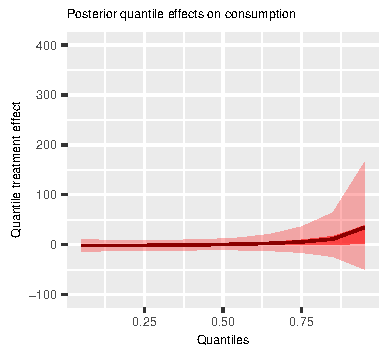
\includegraphics{posterior_parent_quantile_TEs_consumption_lognormal.pdf}
        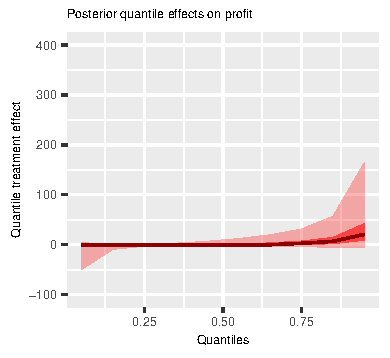
\includegraphics{posterior_parent_quantile_TEs_profit_lognormal.pdf}\\
    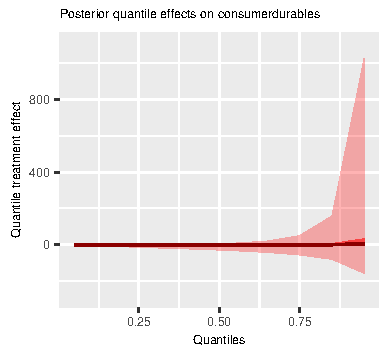
\includegraphics{posterior_parent_quantile_TEs_consumerdurables_lognormal.pdf}
        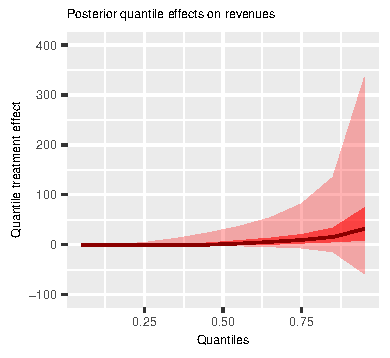
\includegraphics{posterior_parent_quantile_TEs_revenues_lognormal.pdf}\\
    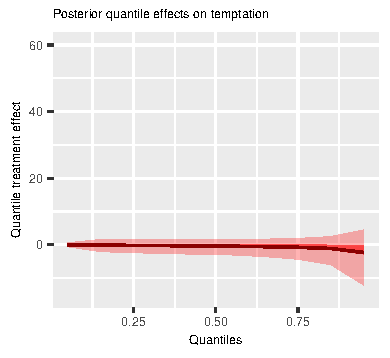
\includegraphics{posterior_parent_quantile_TEs_temptation_lognormal.pdf}
        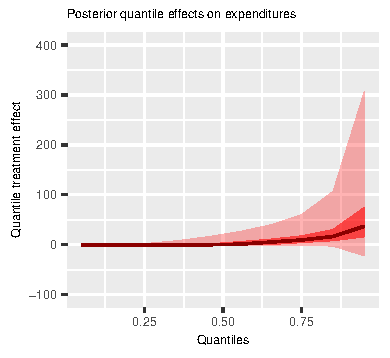
\includegraphics{posterior_parent_quantile_TEs_expenditures_lognormal.pdf}
  \caption{ Average quantile treatment effects in USD PPP per 2 week interval across all settings for all variables. The dark line is the posterior mean, the opaque color bands are the central 50\% posterior uncertainty interval, the translucent color bands are the central 95\% posterior uncertainty interval. }\label{posterior general quantiles}
\end{figure}



%  \hyperref{ posterior predictive quantiles},

 \begin{figure}[h!]
  \centering
   \title{Posterior Predicted Distributions of Extrapolated Quantile Effects In Next Setting}
    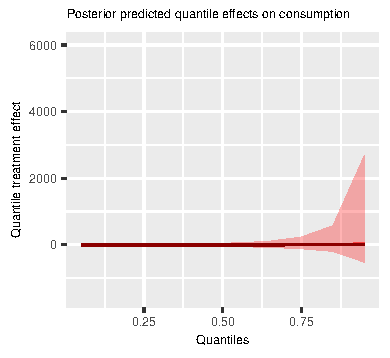
\includegraphics{posterior_predicted_quantile_TEs_consumption_lognormal.pdf}
        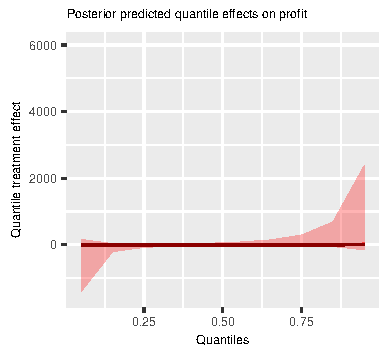
\includegraphics{posterior_predicted_quantile_TEs_profit_lognormal.pdf}\\
    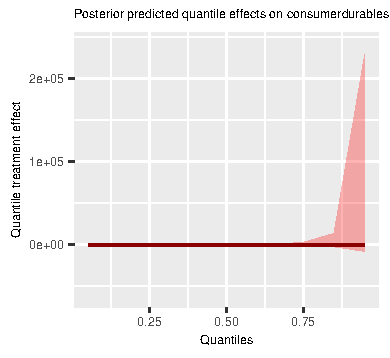
\includegraphics{posterior_predicted_quantile_TEs_consumerdurables_lognormal.pdf}
        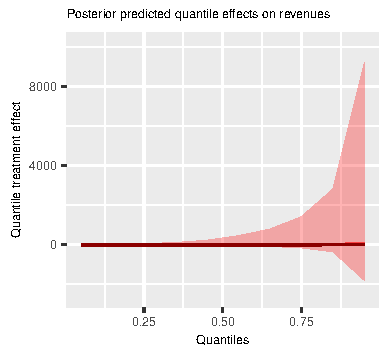
\includegraphics{posterior_predicted_quantile_TEs_revenues_lognormal.pdf}\\
    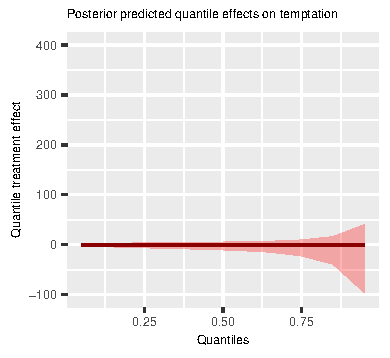
\includegraphics{posterior_predicted_quantile_TEs_temptation_lognormal.pdf}
        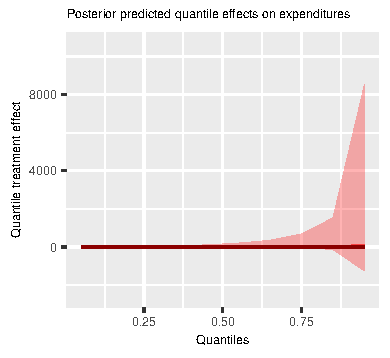
\includegraphics{posterior_predicted_quantile_TEs_expenditures_lognormal.pdf}
  \caption{ Posterior Predictive quantile treatment effects in USD PPP per 2 week interval for the next setting for all variables.The dark line is the posterior mean, the opaque color bands are the central 50\% posterior predictive uncertainty interval, the translucent color bands are the central 95\% posterior predictive uncertainty interval.}\label{posterior predicted quantiles}
\end{figure}

\clearpage

 
  \begin{figure}[h!]
  \centering
  \title{Comparative Model Fit: Lognormal vs Pareto}
    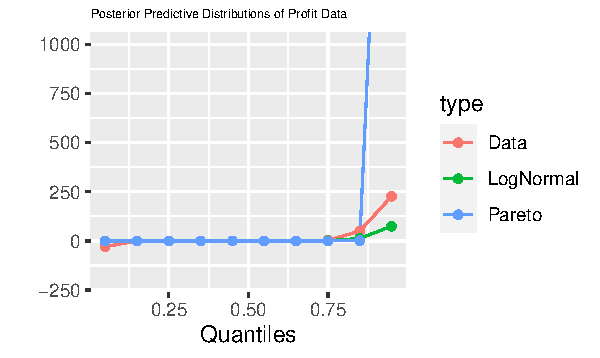
\includegraphics{posterior_predictive_profit.pdf}\\
    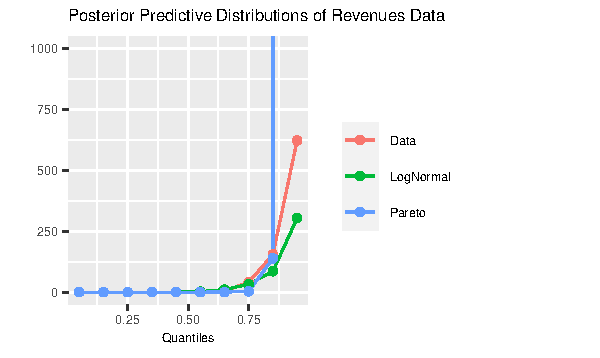
\includegraphics{posterior_predictive_revenues.pdf}\\
          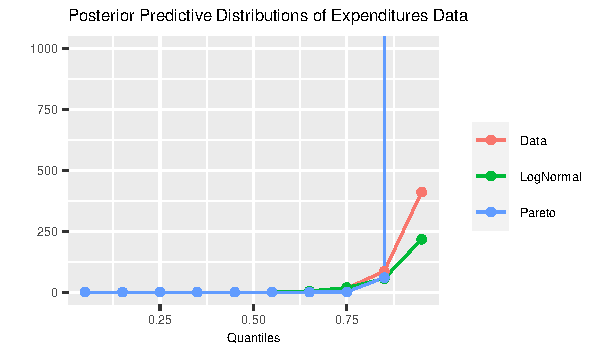
\includegraphics{posterior_predictive_expenditures.pdf}

  \caption{Model fit analysis: posterior predictive quantiles in USD PPP per 2 week interval in the control group from the LogNormal and Pareto models compared to the real data. Further details and caveats can be found in Appendix C. }\label{model fit}
\end{figure}

\clearpage





 %\hyperref{complex models}
 
  \begin{figure}[h!]
  \centering
  \title{Comparative Results of Alternative Tail Shape Models for Profit}
    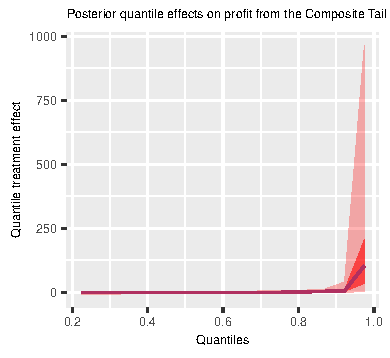
\includegraphics{posterior_parent_quantile_TEs_profit_composite.pdf}\\
    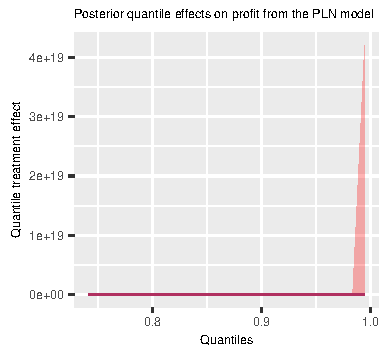
\includegraphics{posterior_parent_quantile_TEs_profit_PLN.pdf}\\
          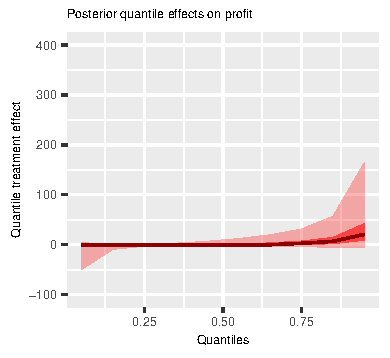
\includegraphics{posterior_parent_quantile_TEs_profit_lognormal.pdf}

  \caption{ \small Average quantile treatment effects in USD PPP per 2 week interval for the next setting for all variables, graphed in square root terms due to the very large scale of the Pareto tail. The dark line is the posterior median, the opaque color bands are the central 50\% posterior predictive uncertainty interval, the translucent color bands are the central 95\% posterior predictive uncertainty interval. The Pareto-Lognormal model has convergence issues as noted in Reed and Jorgensen 2004, here somewhat mitigated by strong priors, and should be interpreted with caution. The Composite tail model, generated by manually cutting up the support of each tail and fitting a Lognormal between zero and the 80th percentile and a Pareto beyond it, is computed in a two-step procedure. Further details and caveats can be found in Appendix C.} \label{complex quantiles}
\end{figure}

\clearpage









%  \hyperref{consumption posterior general quantiles pb split}

 \begin{figure}[h!]
  \centering
  \title{Consumption Variables Quantile Effects split by Prior Business Ownership}
    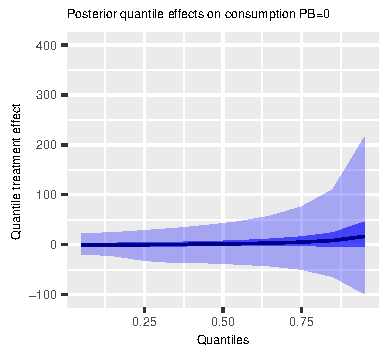
\includegraphics{posterior_parent_quantile_TEs_consumption_pb_0_lognormal.pdf}
    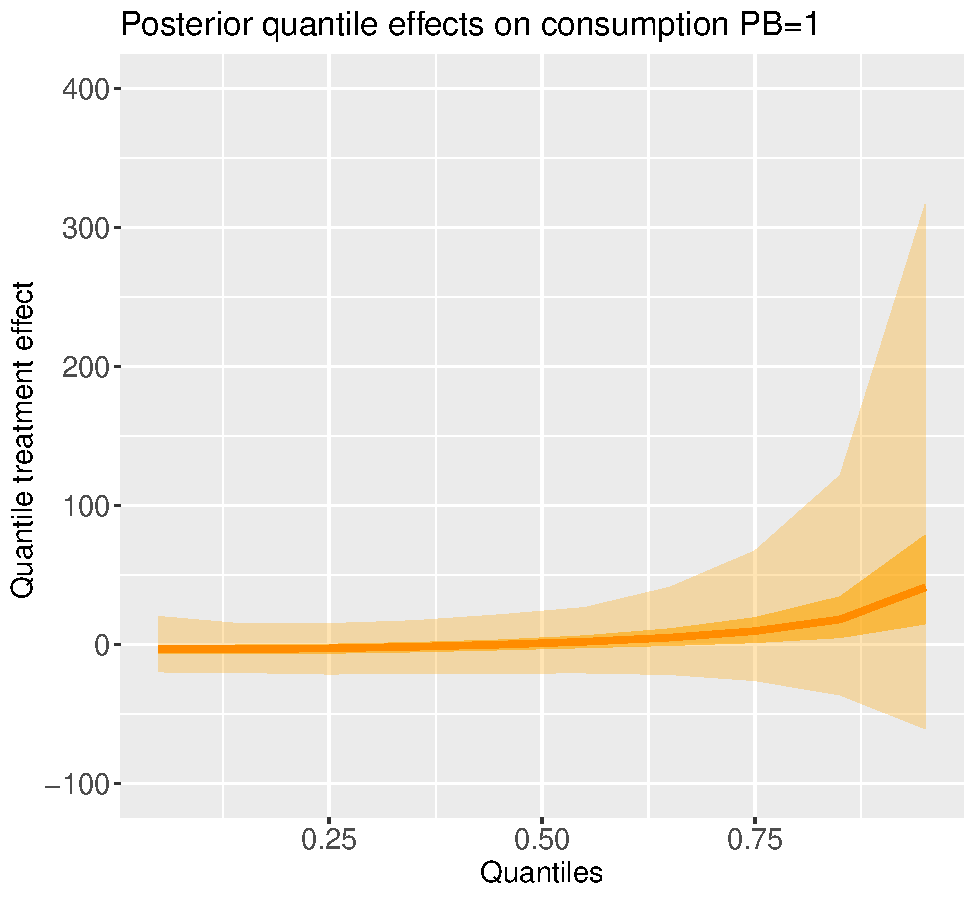
\includegraphics{posterior_parent_quantile_TEs_consumption_pb_1_lognormal.pdf}\\
    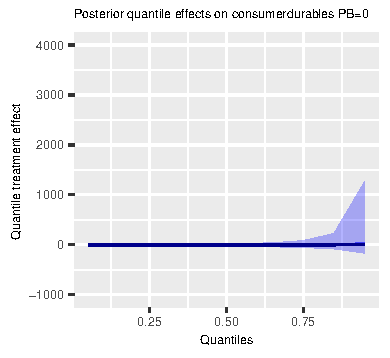
\includegraphics{posterior_parent_quantile_TEs_consumerdurables_pb_0_lognormal.pdf}
    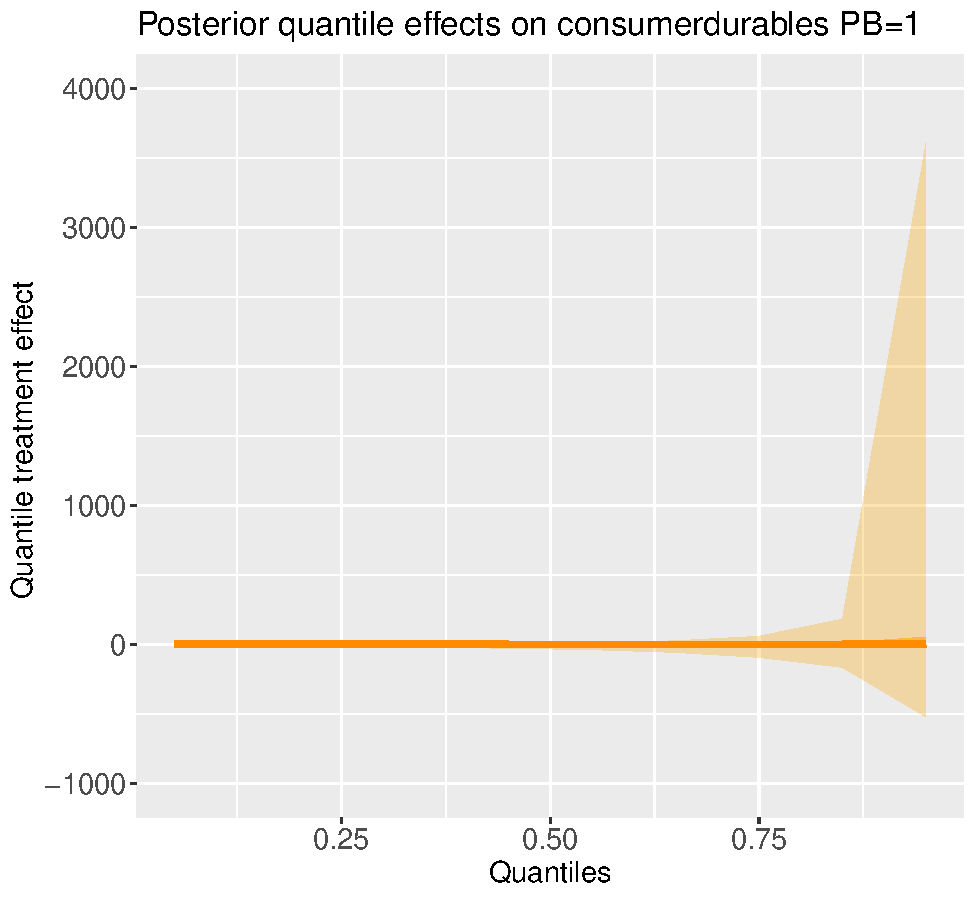
\includegraphics{posterior_parent_quantile_TEs_consumerdurables_pb_1_lognormal.pdf}\\
    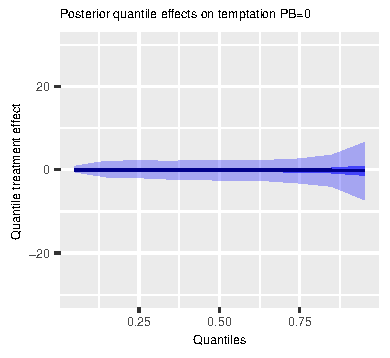
\includegraphics{posterior_parent_quantile_TEs_temptation_pb_0_lognormal.pdf}
    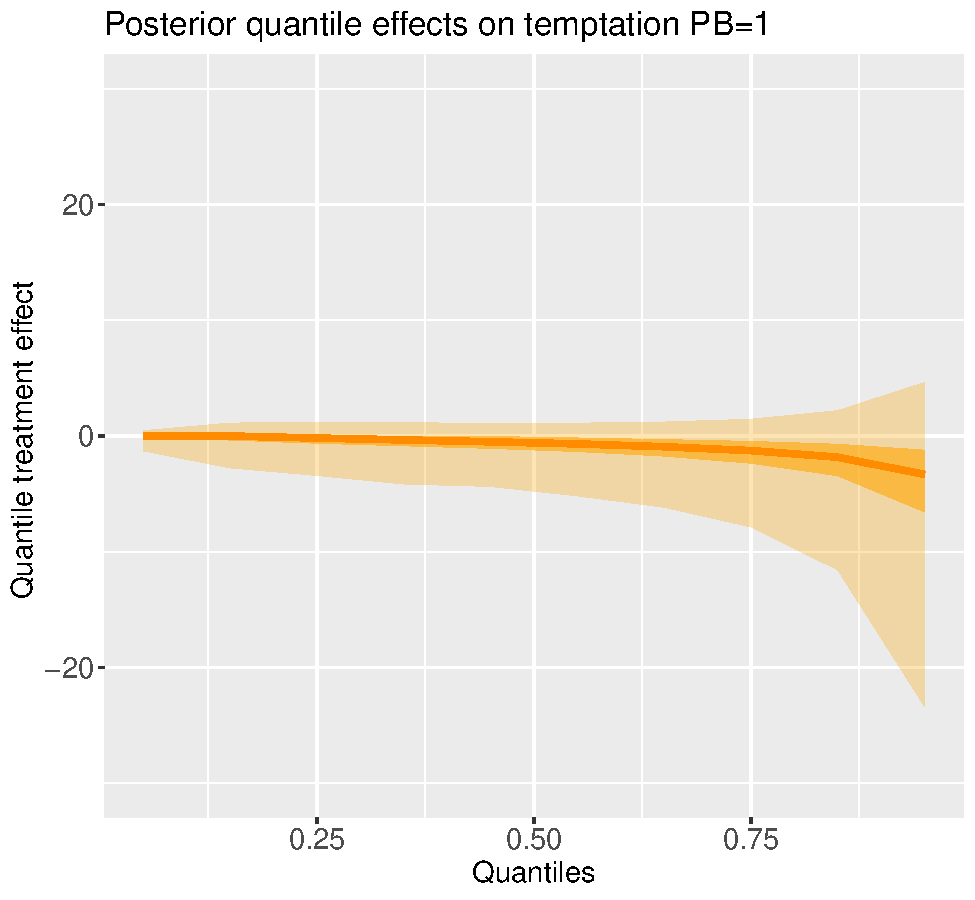
\includegraphics{posterior_parent_quantile_TEs_temptation_pb_1_lognormal.pdf}\\
  \caption{ General Quantile Treatment Effect Curves in USD PPP per 2 week interval split by prior business ownership ($\beta_1$) for consumption-type variables. The dark line is the posterior mean, the opaque color bands are the central 50\% posterior uncertainty interval, the translucent color bands are the central 95\% posterior uncertainty interval. } \label{consumption posterior general quantiles pb split}
\end{figure}


% \hyperref{posterior mean quantiles profit pb split}

 \begin{figure}[h!]
  \centering
    \title{Business Variables Quantile Effects split by Prior Business Ownership}
    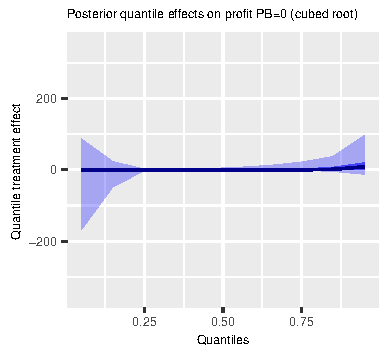
\includegraphics{posterior_parent_quantile_TEs_profit_pb_0_lognormal.pdf}
    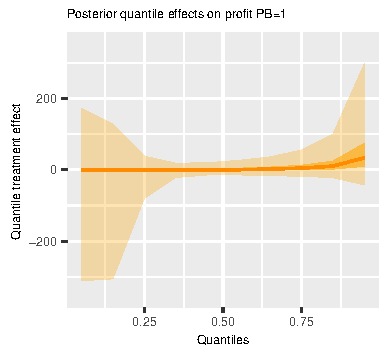
\includegraphics{posterior_parent_quantile_TEs_profit_pb_1_lognormal.pdf}\\
    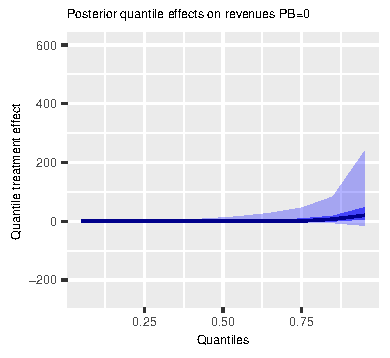
\includegraphics{posterior_parent_quantile_TEs_revenues_pb_0_lognormal.pdf}
    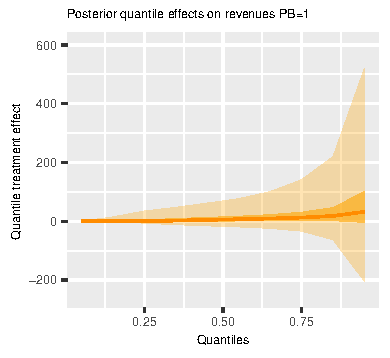
\includegraphics{posterior_parent_quantile_TEs_revenues_pb_1_lognormal.pdf}\\
    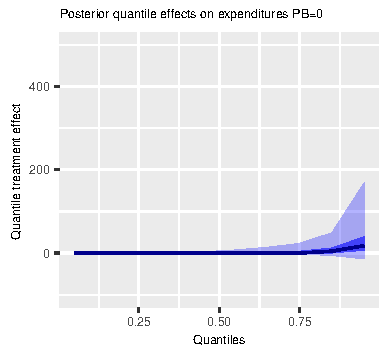
\includegraphics{posterior_parent_quantile_TEs_expenditures_pb_0_lognormal.pdf}
    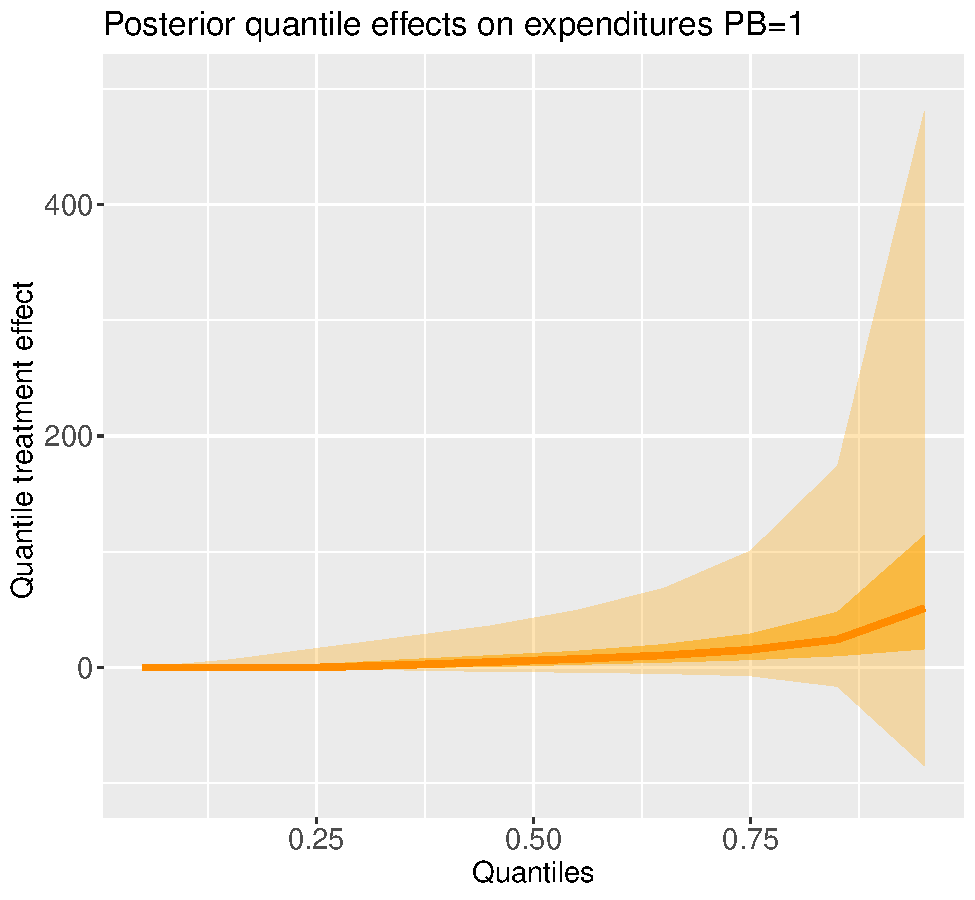
\includegraphics{posterior_parent_quantile_TEs_expenditures_pb_1_lognormal.pdf}
  \caption{ General Quantile Treatment Effect Curves $(\beta_1)$ for business variables split by prior business ownership. The dark line is the median, the opaque bars are the central 50\% interval, the translucent bands are the central 95\% interval. Display is in cubed root of USD PPP per 2 week interval due to the scale differences in the uncertainty at the right tail versus the rest of the distribution. }\label{posterior mean quantiles profit pb split}
\end{figure}









\clearpage \newpage

\begin{thebibliography}{99}

\bibitem{daron} \textbf{Acemoglu, Daron., and James A. Robinson.} 2008. "Persistence of power, elites, and institutions." American Economic Review, 98(1), 267-93.

\bibitem{handbookdaron} \textbf{ Acemoglu, Daron, Suresh Naidu, Pasqual Restrepo, and James A. Robinson.} 2015. "Chapter 21 - Democracy, Redistribution, and Inequality", The Handbook of Income Distribution, Editor(s): Anthony B. Atkinson, Francois Bourguignon, Elsevier, Volume 2, 2015, Pages 1885-1966.

\bibitem{Ahmad} \textbf{ Ahmad, Mokbul Morshed.} 2003. "Distant voices: the views of the field workers of NGOs in Bangladesh on microcredit." The Geographical Journal, 169(1), 65-74.

\bibitem{acac} \textbf{ Albert, Jim, and Siddhartha Chib.} 1997. "Conditionally Independent Hierarchical Models", Journal of the American Statistical Association, September 1997, Vol. 92, No. 439

\bibitem{allcott} \textbf{ Allcott, Hunt.} 2015. "Site Selection Bias in Program Evaluation." The Quarterly Journal of Economics, 130(3), 1117-1165.

\bibitem{allen} \textbf{ Allen, Treb.} 2014. "Information frictions in trade". Econometrica, 82(6), 2041-2083.

\bibitem{emily}\textbf{  Andrews, Isaiah, and Emily Oster.} 2017. "Weighting for External Validity" (No. w23826). National Bureau of Economic Research.

\bibitem{angelucci} \textbf{ Angelucci, Manuela, Dean Karlan, and Jonathan Zinman.} 2015. "Microcredit Impacts: Evidence from a Randomized Microcredit Program Placement Experiment by Compartamos Banco." American Economic Journal: Applied Economics, 7(1): 151-82.

\bibitem{angirst} \textbf{ Angrist, Joshua D.} 2004. "Treatment effect heterogeneity in theory and practice". The Economic Journal, 114(494), C52-C83.

\bibitem{afv} \textbf{ Angrist, Joshua D., and Ivan Fernandez-Val.} 2010. "Extrapolate-ing: External validity and overidentification in the late framework" (No. w16566). National Bureau of Economic Research.

\bibitem{athey} \textbf{ Athey, Susan, and Guido Imbens.} "Recursive partitioning for heterogeneous causal effects." Proceedings of the National Academy of Sciences 113, no. 27 (2016): 7353-7360.

\bibitem{attanasio} \textbf{ Attanasio, Orazio, Britta Augsburg, Ralph De Haas, Emla Fitzsimons, and Heike Harmgart.} 2015. "The Impacts of Microfinance: Evidence from Joint-Liability Lending in Mongolia." American Economic Journal: Applied Economics, 7(1): 90-122.

\bibitem{Augsburg} \textbf{ Augsburg, Britta, Ralph De Haas, R., Heike Harmgart, and Costas Meghir.} 2015. "The Impacts of Microcredit: Evidence from Bosnia and Herzegovina." American Economic Journal: Applied Economics, 7(1): 183-203.

\bibitem{or} \textbf{ Bandiera, Oriana, Greg Fischer, Andrea Prat, and Erina Ytsma.} 2017. "Do Women Respond Less to Performance Pay? Building Evidence from Multiple Experiments" Working Paper Version October 2017

\bibitem{banerjee2013} \textbf{ Banerjee, Abhijit.} 2013. "Microcredit under the microscope: what have we learned in the past two decades, and what do we need to know?". Annu. Rev. Econ., 5(1), 487-519.

\bibitem{banerjee20151} \textbf{ Banerjee, Abhijit, Dean Karlan, and Jonathan Zinman.} 2015a. "Six Randomized Evaluations of Microcredit: Introduction and Further Steps." American Economic Journal: Applied Economics, 7(1): 1-21.

\bibitem{banerjee20152} \textbf{ Banerjee, Abhijit, Esther Duflo, Rachael Glennerster, and Cynthia Kinnan.} 2015b. "The Miracle of Microfinance? Evidence from a Randomized Evaluation." American Economic Journal: Applied Economics, 7(1): 22-53.

\bibitem{banerjeescience} \textbf{ Banerjee, Abhijit, Esther Duflo, Nathaniel Goldberg, Dean Karlan, Robert Osei, William Pariente, Jeremy Shapiro, Bram Thuysbaert, and Christopher Udry.} 2015c. "A multifaceted program causes lasting progress for the very poor: Evidence from six countries." Science 348, no. 6236 (2015): 1260799.

\bibitem{sendhil} \textbf{ Banerjee, Abhijit, and Sendhil Mullainathan.} 2010. "The shape of temptation: Implications for the economic lives of the poor" (No. w15973). National Bureau of Economic Research. NBER Working Paper No. 15973, Issued in May 2010

\bibitem{Bazzi} \textbf{ Bazzi, Samuel.} 2016. "Wealth Heterogeneity and the Income Elasticity of Migration." American Economic Journal: Applied, 9(2), 219-55.

\bibitem{bert} \textbf{ Bertanha, Marinho, and Guido Imbens.} 2014. "External validity in fuzzy regression discontinuity designs" (No. w20773). National Bureau of Economic Research.

\bibitem{betancourt} \textbf{ Betancourt, Michael J., and Mark Girolami.} 2013. "Hamiltonian Monte Carlo for hierarchical models." arXiv preprint arXiv:1312.0906

\bibitem{bisbee}\textbf{  Bisbee, James Hodgdon, Rajeev Dehejia, Christian Pop-Eleches, and Cyrus Samii.} 2016. "Local Instruments, Global Extrapolation: External Validity of the Labor Supply". Journal of Labor Economics, Volume 35, Number S1, pp. S99-S147.

\bibitem{k} \textbf{ Borusyak, Kirill, and Xavier Jaravel.} 2018. "The Distributional Effects of Trade: Theory and Evidence from the United States." Working Paper Version.

\bibitem{bk} \textbf{ Breza, Emily, and Cynthia Kinnan.} 2018. "Measuring the equilibrium impacts of credit: Evidence from the Indian microfinance crisis" (No. w24329). National Bureau of Economic Research

\bibitem{brez} \textbf{ Breza, Emily.} 2012. "Peer effects and loan repayment: Evidence from the Krishna default crisis." Working paper.

\bibitem{Gha} \textbf{ Bryan, Gharad, Shyamal Chowdhury, and Ahmed Mushfiq Mobarak.} 2014. "Underinvestment in a profitable technology: The case of seasonal migration in Bangladesh." Econometrica, 82(5), 1671-1748.

\bibitem{cast} \textbf{ Castellacci, Giuseppe.} 2012. "A Formula for the Quantiles of Mixtures of Distributions with Disjoint Supports". Available at SSRN: http://ssrn.com/abstract=2055022 or http://dx.doi.org/10.2139/ssrn.2055022

\bibitem{chern} \textbf{ Chernozhukov, Victor V., Ivan Fernandez-Val, and Alfred Galichon.} 2010. "Quantile and probability curves without crossing." Econometrica 78.3  1093-1125.

\bibitem{chetty} \textbf{ Chetty, Raj, Nathaniel Hendren, and Lawrence F. Katz.} 2016. "The effects of exposure to better neighborhoods on children: New evidence from the Moving to Opportunity experiment." American Economic Review, 106(4), 855-902.

\bibitem{rchetz} \textbf{ Chetty, Raj, and Nathaniel Hendren.} 2018. "The impacts of neighborhoods on intergenerational mobility I: Childhood exposure effects." The Quarterly Journal of Economics, 133(3), 1107-1162.

\bibitem{chet} \textbf{ Chetty, Raj, John N. Friedman, and Jonah E. Rockoff.} 2014. "Measuring the impacts of teachers I: Evaluating bias in teacher value-added estimates." American Economic Review, 104(9), 2593-2632

\bibitem{sid} \textbf{ Chib, Siddhartha, and Edward Greenberg.} 1995. "Hierarchical analysis of SUR models with extensions to correlated serial errors and time-varying parameter models." Journal of Econometrics, 68(2), 339-360.

\bibitem{Chung1} \textbf{ Chung, Yeojin, Andrew Gelman, Sophia Rabe-Hesketh, Jingchen Liu, and Vincent Dorie.} 2015. Weakly informative prior for point estimation of covariance matrices in hierarchical models. Journal of Educational and Behavioral Statistics, 40(2), 136-157.

\bibitem{Chung2} \textbf{ Chung, Yeojin, Sophia Rabe-Hesketh, Vincent Dorie, Andrew Gelman, and Jingchen Liu.} 2013. "A nondegenerate penalized likelihood estimator for variance parameters in multilevel models." Psychometrika, 78(4), 685-709.

\bibitem{comp} \textbf{ Compiani, Giovanni, and Yuichi Kitamura.} 2016. "Using mixtures in econometric models: a brief review and some new results." Econometrics Journal, 19, C95-C127.

\bibitem{crepon} \textbf{ Crepon, Bruno, Florence Devoto, Esther Duflo, and William Pariente.} 2015. "Estimating the Impact of Microcredit on Those Who Take It Up: Evidence from a Randomized Experiment in Morocco." American Economic Journal: Applied Economics, 7(1): 123-50.

\bibitem{dehe} \textbf{ Dehejia, Rajeev, Christian Pop-Eleches, and Cyrus Samii.} 2015. "From Local to Global: External Validity in a Fertility Natural Experiment" (No. w21459). National Bureau of Economic Research.

\bibitem{de} \textbf{ Dehejia, Rajeev. H.} 2003. "Was there a Riverside miracle? A hierarchical framework for evaluating programs with grouped data." Journal of Business \& Economic Statistics, 21(1), 1-11.

\bibitem{Diaconis} \textbf{ Diaconis, Persi.} 1977. "Finite Forms of De Finetti's Theorem on Exchangeability" Synthese, 36, 1977,  271-281

\bibitem{duflo} \textbf{ Duflo, Esther, Pascaline Dupas, and Michael Kremer.} 2017 "The Impact of Free Secondary Education: Experimental Evidence from Ghana" Working Paper, 2017

\bibitem{efron} \textbf{ Efron, Bradley, and Carl Morris.} 1975. "Data analysis using Stein's estimator and its generalizations". Journal of the American Statistical Association, 70(350), 311-319.

\bibitem{fink} \textbf{ Fink, Gunther, B. Kelsey Jack, and Felix Masiye.} 2014. Seasonal credit constraints and agricultural labor supply: Evidence from Zambia (No. w20218). National Bureau of Economic Research.

\bibitem{gabaix} \textbf{ Gabaix, Xavier.} 2008. "Power Laws in Economics and Finance" NBER Working Paper No. 14299, accessed online August 12th 2016, http://www.nber.org/papers/w14299

\bibitem{gech} \textbf{ Gechter, Michael.} 2015. "Generalizing the Results from Social Experiments: Theory and Evidence from Mexico and India". manuscript, Pennsylvania State University.

\bibitem{bda} \textbf{ Gelman, Andrew, John Carlin, Hal Stern, David Dunson, Aki Vehtari and Donald Rubin.} 2004. "Bayesian Data Analysis: Second Edition", Taylor \& Francis

\bibitem{GP} \textbf{Gelman, Andrew and Ian Pardoe.} 2006. "Bayesian measures of explained variance and pooling in multilevel (hierarchical) models." Technometrics, 48(2), pp.241-251.

\bibitem{hall} \textbf{ Hall, Peter, and Xiao-Hua Zhou.} 2003. Nonparametric estimation of component distributions in a multivariate mixture. The annals of statistics, 31(1), 201-224.

\bibitem{nat} \textbf{ Hussam, Reshmann, Natalia Rigol, and Benjamin Roth.} 2017. "Targeting high ability entrepreneurs using community information: Mechanism design in the field." MIT Working Paper, November 2017.

\bibitem{hastie} \textbf{ Hastie, Trevor, Robert Tibshirani, and Jerome Friedman.} 2009. "The elements of statistical learning". Second Edition. Springer Series in Statistics.

\bibitem{heck} \textbf{ Heckman, James, Justin L. Tobias, and Edward Vytlacil.} 2001. "Four parameters of interest in the evaluation of social programs". Southern Economic Journal, 211-223.

\bibitem{ghoff} \textbf{ Hoffman, Matthew D., and Andrew Gelman.} 2014."The no-U-turn sampler: Adaptively setting path lengths in Hamiltonian Monte Carlo". The Journal of Machine Learning Research, 15(1), 1593-1623.

\bibitem{burke} \textbf{ Hsiang, Solomon. M., Marshall Burke, and Edward Miguel.} 2013. "Quantifying the influence of climate on human conflict." Science, 341(6151), 1235367.

\bibitem{phull} \textbf{ Hull, Peter.} 2018. "Estimating hospital quality with quasi-experimental data." University of Chicago Working Paper.

\bibitem{kaboski} \textbf{ Kaboski, Joseph P., and Robert Townsend.} 2011. "A structural evaluation of a large-scale quasi-experimental microfinance initiative". Econometrica, 79(5), 1357-1406.

\bibitem{SA} \textbf{ Karlan, Dean, and Jonathan Zinman.} 2009. "Observing unobservables: Identifying information asymmetries with a consumer credit field experiment." Econometrica, 77(6), 1993-2008.

 \bibitem{karlan} \textbf{ Karlan, Dean, and Jonathan Zinman, J.} 2011. "Microcredit in Theory and Practice: Using Randomized Credit Scoring for Impact Evaluation", Science 10 June 2011: 1278-1284
 
 \bibitem{kasahar} \textbf{ Kasahara, Hiroyuki., and Katsumi Shimotsu.} 2009. "Nonparametric identification of finite mixture models of dynamic discrete choices." Econometrica, 77(1), 135-175.
 
\bibitem{kin} \textbf{ Kinnan, Cynthia, and Robert Townsend.} 2012. "Kinship and financial networks, formal financial access, and risk reduction." American Economic Review, 102(3), 289-93.

\bibitem{KB} \textbf{ Koenker, Roger, and Gilbert Basset.} 1978. "Regression Quantiles"  Econometrica, Vol. 46, No. 1. (Jan., 1978), pp. 33-50.

\bibitem{Kh} \textbf{ Koenker, Roger, and Kevin F. Hallock.} 2001. "Quantile Regression." Journal of Economic Perspectives, 15(4): 143-156

\bibitem{leon} \textbf{ Leon, Andrew C., and Moonseong Heo.} 2009. "Sample Sizes Required to Detect Interactions between Two Binary Fixed-Effects in a Mixed-Effects Linear Regression Model." Computational Statistics \& Data Analysis, 53(3), 603?608.

\bibitem{machado} \textbf{ Machado, Jose A.F, and J. M. C. Santos Silva.} 2005. "Quantiles for Counts" Journal Of The American Statistical Association Vol. 100 , Iss. 472

\bibitem{karen} \textbf{ Macours, Karen, and Renos Vakis.} 2010. "Seasonal migration and early childhood development". World development, 38(6), 857-869.

\bibitem{mcculloch} \textbf{ McCulloch, Charles E., and John M. Neuhaus.} 2011. "Misspecifying the Shape of a Random Effects Distribution: Why Getting It Wrong May Not Matter". Statist. Sci. 26 (2011), no. 3, 388--402.

\bibitem{macca} \textbf{ Gibson, John., and David McKenzie.} 2014. "The development impact of a best practice seasonal worker policy." Review of Economics and Statistics, 96(2), 229-243.

\bibitem{miller} \textbf{ Miller, Jeffrey W., and Matthew T. Harrison.} 2013. "A simple example of Dirichlet process mixture inconsistency for the number of components." In?Advances in neural information processing systems?(pp. 199-206).

\bibitem{meager} \textbf{ Meager, Rachael.} 2019. "Understanding the average impact of microcredit expansions: A Bayesian hierarchical analysis of seven randomized experiments." American Economic Journal: Applied Economics, 11(1), 57-91.

\bibitem{Micro} \textbf{ Microfinance Barometer.} 2020. "Microfinance Barometer 10th Edition: 10 Years Already", Convergences, France, www.convergences.org, 2020

\bibitem{Microfinance Focus} \textbf{ Microfinance Focus}. 2011. "Six Microfinance Crises the sector does not want to remember." http://www.microfinancefocus.com/6-microfinance-crises-sector-does-not-want-remember

\bibitem{morduch} \textbf{ Morduch, Jonathan.} 1999. "The microfinance promise." Journal of economic literature, 37(4), 1569-1614.

\bibitem{Mosteller} \textbf{ Mosteller, Frederick.} 1946. "On Some Useful "Inefficient" Statistics" The Annals of Mathematical Statistics, Vol. 17, No. 4. (Dec., 1946), pp. 377-408

\bibitem{pik} \textbf{ Piketty, Thomas.} 2015. "About capital in the twenty-first century." American Economic Review, 105(5), 48-53.

\bibitem{pritchettsandefur} \textbf{ Pritchett, Lant, and Justin Sandefur.} 2015. "Learning from Experiments when Context Matters"  American Economic Association 2015 Preview Papers, accessed online February 2015

\bibitem{reed} \textbf{ Reed, William J., and Jorgensen, Murray.} 2004. The double Pareto-lognormal distribution - a new parametric model for size distributions. Communications in Statistics-Theory and Methods, 33(8), 1733-1753.

\bibitem{roodman} \textbf{ Roodman, David.} 2012. "Due diligence: An impertinent inquiry into microfinance". CGD Books.

\bibitem{roy} \textbf{ Roy, Andrew. D.} 1950. "The distribution of earnings and of individual output." The Economic Journal, 60(239), 489-505.

\bibitem{rubin81} \textbf{ Rubin, Donald. B.} 1981. "Estimation in parallel randomized experiments. Journal of Educational and Behavioral Statistics", 6(4), 377-401.

\bibitem{sch} \textbf{ Schicks, Jessica}. 2013. "From a supply gap to a demand gap? The risk and consequences of over-indebting the underbanked." In Microfinance in Developing Countries (pp. 152-177). Palgrave Macmillan, London.

\bibitem{stan} \textbf{ Stan Development Team}. 2017. "Stan Modeling Language: User's Guide and Reference Manual." Version 2.17.0.

\bibitem{stig} \textbf{ Stiglitz, Joseph. E.} 1969. "Distribution of income and wealth among individuals." Econometrica: Journal of the Econometric Society, 382-397.

\bibitem{tarozzi} \textbf{ Tarozzi, Alessandro, Jaikishan Desai, and Kristen Johnson. }2015. "The Impacts of Microcredit: Evidence from Ethiopia." American Economic Journal: Applied Economics, 7(1): 54-89.

\bibitem{vivalt} \textbf{ Vivalt, Eva.} 2016. "How much can we generalise from impact evaluations?" Working Paper, NYU

\bibitem{vandervaart} \textbf{ Van der Vaart, Aad. W.} 1998. "Asymptotic Statistics", Cambridge Series in Statistical and Probabilistic Mathematics, Cambridge University Press

\bibitem{yunus} \textbf{ Yunus, Mohammed.} 2006. "Nobel Lecture", Oslo, December 10, 2006.


\end{thebibliography}





\end{document}

